% The master copy of this demo dissertation is held on my filespace
% on the cl file serve (/homes/mr/teaching/demodissert/)

% Last updated by MR on 2 August 2001

\documentclass[12pt,notitlepage]{report}

\usepackage{a4}
\usepackage{verbatim}

\usepackage{amsmath}
\usepackage{amssymb}
\usepackage{mathtools}

\usepackage{dirtree}

\usepackage{minted}
%\usemintedstyle{colorful}
\setmintedinline{breaklines}

\usepackage{pgfplots}
\pgfplotsset{compat=1.8}
\usepgfplotslibrary{statistics}

\newcommand{\textinline}{\mintinline{text}}
\newcommand{\cinline}{\mintinline{C}}
\newcommand{\camlinline}{\mintinline{OCaml}}
\newcommand{\wainline}{\mintinline{LISP}}

\newcommand{\cfbox}[2]{%
	\colorlet{currentcolor}{.}%
	{\color{#1}%
		\fbox{\color{currentcolor}#2}}%
}
\newcommand\note[1]{\noindent\cfbox{blue}{\parbox{\textwidth}{\textcolor{blue}{#1}}}}
%\newcommand\note[1]{}

%\input{epsf}                            % to allow postscript inclusions
% On thor and CUS read top of file:
%     /opt/TeX/lib/texmf/tex/dvips/epsf.sty
% On CL machines read:
%     /usr/lib/tex/macros/dvips/epsf.tex



\raggedbottom                           % try to avoid widows and orphans
\sloppy
\clubpenalty1000%
\widowpenalty1000%

\addtolength{\oddsidemargin}{6mm}       % adjust margins
\addtolength{\evensidemargin}{-8mm}

\renewcommand{\baselinestretch}{1.1}    % adjust line spacing to make
                                        % more readable

\usepackage[backend=bibtex, style=alphabetic, sorting=ynt]{biblatex}
\addbibresource{refs.bib}

\begin{document}



%%%%%%%%%%%%%%%%%%%%%%%%%%%%%%%%%%%%%%%%%%%%%%%%%%%%%%%%%%%%%%%%%%%%%%%%
% Title


\pagestyle{empty}

\hfill{\LARGE \bf Paul Durbaba}

\vspace*{60mm}
\begin{center}
\Huge
{\bf Compiling OCaml to WebAssembly} \\
\vspace*{5mm}
Computer Science Tripos Part II \\
\vspace*{5mm}
Robinson College \\
\vspace*{5mm}
May 2020  % today's date
\end{center}

\clearpage


 
\newpage
\section*{Declaration}

I, Paul Durbaba of Robinson College, being a candidate for Part II of the Computer
Science Tripos, hereby declare
that this dissertation and the work described in it are my own work,
unaided except as may be specified below, and that the dissertation
does not contain material that has already been used to any substantial
extent for a comparable purpose.

\bigskip
\leftline{Signed Paul Durbaba}

\medskip
\leftline{Date [date]}

\section*{Acknowledgements}

% TODO List the people that check the diss
\note{LIST THE PEOPLE THAT CHECK THE DISS}

%%%%%%%%%%%%%%%%%%%%%%%%%%%%%%%%%%%%%%%%%%%%%%%%%%%%%%%%%%%%%%%%%%%%%%%%%%%%%%
% Proforma, table of contents and list of figures

\setcounter{page}{1}
\pagenumbering{roman}
\pagestyle{plain}

\chapter*{Proforma}

{\large
	\begin{tabular}{ll}
		Name:               & \bf Paul Durbaba                       \\
		College:            & \bf Robinson College                     \\
		Project Title:      & \bf Compiling OCaml to WebAssembly \\
		Examination:        & \bf Part II Computer Science, May 2020        \\
		Word Count:         & \bf FILL IN LATER, CURRENTLY 13K  \\
		Project Originator: & Timothy M. Jones                \\
		Supervisor:         & Tobias Kohn            \\ 
	\end{tabular}
}
%\footnotetext[1]{This word count was computed
%	by {\tt detex diss.tex | tr -cd '0-9A-Za-z $\tt\backslash$n' | wc -w}
%}
%\stepcounter{footnote}


\section*{Original Aims of the Project}

\note{At most 100 words describing the original aims of the project.}


\section*{Work Completed}

\note{At most 100 words summarising the work completed.}

\section*{Special Difficulties}

\note{At most 100 words describing any special difficulties that you faced.
(In most cases the special difficulties entry will say “None”.) }
None.

\tableofcontents

\listoffigures

%%%%%%%%%%%%%%%%%%%%%%%%%%%%%%%%%%%%%%%%%%%%%%%%%%%%%%%%%%%%%%%%%%%%%%%
% now for the chapters

\clearpage        % just to make sure before the page numbering
                        % is changed

\setcounter{page}{1}
\pagenumbering{arabic}
\pagestyle{headings}

\chapter{Introduction}

%\note{The Introduction should explain the principal motivation for the project. Show how the work fits into the broad area of surrounding Computer Science and give a brief survey of previous related work. It should generally be unnecessary to quote at length from technical papers or textbooks. If a simple bibliographic reference is insufficient, consign any lengthy quotation to an appendix.}
%TODO EXPLAIN KEY MOTIVATION, IDEAS BEHIND PROJECT
My motivation for this project is to learn how to make a compiler. Compilers are essential to computing because they enable the transformation of code from high-level languages that are intuitive for use by us, into low-level machine understandable code than can actually be executed, and writing a compiler is a substantial software project that invokes many areas of computer science such as type theory and program analysis.

% TODO PREVIOUS RELATED WORK

\section{OCaml}
OCaml\cite{OCaml} is a strongly-typed functional programming language, with some imperative features such as references. I chose OCaml both as the source language of the compiler, and the language the compiler is designed in, because I wanted to gain some familiarity in writing programs in functional languages, and OCaml has similar syntax to Standard ML taught in first year, but with much better library support, and because compiling a functional programming language presents additional challenges to compiling an imperative language such as C - with first class functions and pattern matching requiring special consideration.

\section{WebAssembly}
% copied from project proposal
WebAssembly\cite{webassembly} is a stack-based binary instruction format for the web. It is not a replacement of JavaScript, instead working alongside JavaScript with the main goal of improving the performance of  more computationally intensive functions in web applications, leaving tasks like DOM manipulation to JavaScript (there are no plans for WebAssembly to support this) It  is  expected  that  a  JavaScript  application might  call  some  functions  implemented  in  WebAssembly  to  perform  computation,  and then display the results itself.
\\\\
WebAssembly was chosen as the target instruction set because it is relatively new, with few compilers out there currently targeting it, and it is likely to grow in popularity in the future as more extensions are added to it that make it more viable to be used - such as support for garbage collection and exceptions.

% TODO

%TODO WHAT IS WEBASSEMBLY


% TODO DESCRIPTION OF HOW TO BUILD THE PROJECT?

\section{Related Work}
% TODO Js\_of\_ocaml, A

There have been a few attempts to compile OCaml to WebAssembly already, such as by @SanderSpies\cite{Awbfo}, who modified the existing backend of the OCaml Compiler to target WebAssembly. Their attempt worked from the `CMM' --- the final stage of the OCaml compiler before code generation, modifying that to include extra type information for WebAssembly, and then doing code generation. This differs from my approach in that I have implemented almost an entire compiler from the type-checker through to the WebAssembly code generator, but excluding lexing/parsing.
\\\\
While Sander's approach allows them to leverage the existing features and optimisations of the OCaml compiler, their approach didn't fit with my goals of learning how to write an entire compiler - such an approach wouldn't give me the freedom and opportunity to explore aspects of compiler construction such as type-checking, intermediate representations, and optimisations, which are some of the most interesting parts of the project.
\clearpage

\chapter{Preparation}
%\note{The chapter will cite any new programming languages and systems which had to be learnt and will mention complicated theories or algorithms which required understanding.}

%\note{It is essential to declare the Starting Point (see Section 7). This states any existing codebase or materials that your project builds on. The text here can commonly be identical to the text in your proposal, but it may enlarge on it or report variations. For instance, the true starting point may have turned out to be different from that declared in the proposal and such discrepancies must be explained. }

\section{Requirements}
The success criteria in the project proposal presented a clearly defined subset of OCaml to implement. This subset was designed to be large enough so that useful OCaml programs could be written in it, while small enough that it was feasible to implement by Christmas.
\\\\
In addition, a set of code samples was needed to test the compiler. I decided to build up this set of samples over the course of the implementation, as I could better consider where the edge cases might lie after I had developed an implementation to test.
\\\\
The proposal also suggested that I construct some kind of browser framework to test these samples, but I later decided that a NodeJS environment would be a more practical and easier automated solution to testing.

% TODO STARTING POINT

% TODO MATERIAL DONE BEFORE CODE WAS WRITTEN

% TODO? HOW I ENSURED CODING WASN'T TRIAL AND ERROR

\section{WebAssembly}
%\note{TODO Move WebAssembly stuff from introduction to here, give overview of features e.g. limited stack manipulation, variables, verified}
The current MVP (minimum viable product) version of WebAssembly is designed for compiled languages like C and C++ that do not use garbage collection and can make do without exceptions. There are extensions currently being developed to add support for these features, but progress on these is slow as they often depend on other extensions, for instance the garbage collection extension depends on extensions for reference types and typed function references, which seek to expand the WebAssembly type system so for instance a garbage collector would understand the shape of data in memory\cite{Wgce}.
\\\\
There are a few interesting features of WebAssembly which are worth drawing attention to:
\begin{itemize}
    \item WebAssembly instructions operate on a stack, however stack manipulation is limited. For instance, there are no instructions to duplicate the top of the stack or swap the top two elements. Instead, functions may specify local variables, and there are instructions to load/save these to/from the stack.
    \item WebAssembly modules are verified before they are executed. This verification traces what will be on the stack, ensuring for instance that there are enough values on the stack to execute each instruction. The types of these values are also verified, ensuring that a function of type \wainline{i32} does not return a value of \wainline{f32} or even no value if the stack was empty.
    \item Limited branching is available. It is only possible to branch to the end of `blocks' and the beginning of `loops'.
    \item The JavaScript interface can only pass \wainline{i32} and \wainline{f32/f64} values to/from WebAssembly functions. There is no way to pass in 64-bit integers as they are unsupported in JavaScript, hence I used 32-bit integers only. To keep things simple I also restricted my implementation to 32-bit floating point values since they can both fit in the same amount of memory.
\end{itemize}

%\note{TODO Alan suggests moving to Preparation, and giving an overview of WA's linguistic features. I already have a bit of an overview in the code generation section, but these are the main ones:
%    \begin{itemize}
%        \item Stack based, structured (but compiler doesn't use this structure much / goes for unstructured options)
%        \item Local variables get/set/tee
%        \item No swap or dup instructions
%        \item Verified i32/f32 types, must know signature of function for all function calls, blocks have a result type
%        \item Can branch only out of a block early, or to the start of a loop
%        \item JS interface can only pass i32 and f32 values - no strings / structs or anything
%\end{itemize}}

\section{Components of the Compiler}
This section provides a very brief overview of each component of the compiler. Full descriptions of what each component does are provided in the implementation.

\subsection{Front End}
The Front End performs lexing and parsing using the OCaml compiler's lexer and parser. Lexing converts a file into a stream of tokens, and parsing converts this stream of tokens into an Abstract Syntax Tree (AST) --- representing the structure of the OCaml code.

\subsection{Type Inference}
The type-inference stage converts the AST into a typed-AST, providing each node in the AST with a type. This is achieved using a Hindley-Milner based type-inference algorithm, producing a set of type-constraints and solving them to produce the final types of each node.

\subsection{Lambda Lifting / Closure Conversion}
Lambda Lifting is the process of converting nested functions to top-level functions: additional parameters are added to represent variables in-scope at the nested-function definition. Closure conversion then replaces the original definition sites of these functions with the creation of `closure' objects: a closure contains the needed environment variables to execute the function --- they provide a way of passing around function references that can be executed without the required variables in the function going out of scope.
\\\\
My compiler performs both of these, producing a list of functions alongside a modified top-level AST.

\subsection{Direct Call Generation and Tail Call Optimisation}
Direct Call Generation is an optimisation that `undoes' some of the closure conversion, inserting direct calls where possible to avoid the overhead of closures. Tail Call Optimisation converts tail-recursive functions to use loops, making tail-recursion safe to use with no risk of stack-overflow. This section was implemented as an extension.

\subsection{Intermediate Translation}
Intermediate Translation serves to transform the AST into an `Intermediate Representation' (IR) --- a language designed to act as an intermediate between the source language and target language. My IR is an instruction set that eliminates features such as patterns and expressions and replaces them with a sequence of basic instructions, using variables to pass values between instructions.

\subsection{IR Optimisations}
I implemented a group of data-flow optimisations as an extension. These serve to improve the IR code in terms of time efficiency, memory usage or number of instructions.

\subsection{Code Generation}
Code Generation is the process of generating target language code from the final IR. My compiler produces a WebAssembly Text Format file. The code generator must take into account the differences between the IR and the target language --- instructions in my IR operate on variables, while WebAssembly instructions operate on the stack with special instructions for loading and saving variables. To meet the success criteria, I implemented a naive solution that made excessive use of these special load/save variable instructions. I later implemented an improved code generator that makes better use of the WebAssembly stack as an extension.

\section{Libraries Used}
\subsection{OCaml Compiler Libs}
I used the official OCaml compiler \cite{OCaml} libraries to perform lexing and parsing, which provide the same frontend as used by the official OCaml compiler. As the frontend of the official OCaml compiler is liable to change between releases, I stuck to version 4.08, which was the most recent version when I started the project but has now been succeeded by 4.09.

\subsection{WebAssembly Binary Toolkit}
The WebAssembly Binary Toolkit \cite{Wabt} (WABT)  is a separate tool which can compile WebAssembly Text Form (.wast files) outputted by my compiler to the WebAssembly Binary Format (.wasm files) that can be loaded by NodeJS and browsers.
\\\\
\note{TODO Explain how to use compiler, then invoke WABT, and then explain JS code to load the WASM? The E2E tester does this so could also be explained in Evaluation chapter?}


\section{Working Environment and Tools Setup}
Since I have both a laptop and desktop, I decided the best way to work on both would be to do the work remotely via a remote desktop application on a remote server. Both my laptop and desktop were configured to download backups from the server once per hour (if they were on), so if there proved to be a problem with the server, I could redeploy easily by uploading the backups to a new server if required.
\\\\
In addition, I used Git in order to keep a record of my work, to allow me to access previous versions of files, and to backup to GitHub

\subsection{Dune}
I chose to use the Dune \cite{Dune} build system for OCaml as it is the most widely-used build system for OCaml, and supports multi-module projects and dependencies installed via OPAM, the OCaml Package Manager.

\subsection{Using The Compiler}
To use the compiler, the OCaml Package Manager opam \cite{Opam} must be installed. The file \textinline{tested-packages.txt} provides a list of all OPAM packages I had installed when testing the compiler. With those packages installed, the script \textinline{build.sh} can be used to build the compiler. This outputs the native executable to \textinline{_build/default/toplevel.exe}.
\\\\
Invoking this executable with the path to an OCaml file ending in \textinline{.ml} will output the corresponding WebAssembly Text Format file to the same path ending in \textinline{.wast}, which can then be compiled using the WebAssembly Binary Toolkit with the command \textinline{wat2wasm}. The outputted WebAssembly Binary Format file will end in \textinline{.wasm}, which can then be loaded and executed in a JavaScript environment. Further details on running WebAssembly modules is available at \cite{Load_wasm}.


\section{Starting Point}
I had very little OCaml experience prior to this project, and experience of writing compilers. In addition, I had no experience of using WebAssembly, but I have plenty of experience writing JavaScript.
\\\\
I attempted to deal with some of these issues prior to starting the project by coming up with some OCaml samples for the compiler to compile in the future, and by setting up an OCaml workspace where I successfully figured out how to import the OCaml Compiler libraries, and learned to navigate the AST they use by writing a simple example that adds one to integer constants. I also read through the WebAssembly documentation to get a sense of which features would be a challenge to compile to WebAssembly.
\clearpage

\chapter{Implementation}
%\note{This chapter should describe what was actually produced: the programs which were written, the hardware which was built or the theory which was developed. Any design strategies that looked ahead to the testing stage might profitably be referred to (the professional approach again).}
%
%\note{Descriptions of programs may include fragments of high-level code but large chunks of code are usually best left to appendices or omitted altogether. Analogous advice applies to circuit diagrams.}
%
%\note{Draw attention to the parts of the work which are not your own. The Implementation Chapter should include a section labelled "Repository Overview". The repository overview should be around one page in length and should describe the high-level structure of the source code found in your source code Repository. It should describe whether the code was written from scratch or if it built on an existing project or tutorial. Making effective use of powerful tools and pre-existing code is often laudable, and will count to your credit if properly reported.}
%
%\note{It should not be necessary to give a day-by-day account of the progress of the work but major milestones may sometimes be highlighted with advantage. }

% TODO WORK DONE, ONE SECTION PER PART OF THE COMPILER

\note{I have a large number of pending comments on this chapter from Tobias, so I expect it's going to have significant rewrites. I've been focusing on the Evaluation and Conclusion recently.}

\section{Front End}
Lexing and parsing is handled by the OCaml Compiler Libs, which produces a \textinline{structure} object representing the AST of the entire program. This AST and the corresponding typed-AST, which I designed to be very similar (using the same names prefixed with a t), are used throughout the first half of the compilation process before intermediate translation occurs. Figure \ref{fig:ast} gives the grammar of the OCaml AST in Extended Backus-Naur form \cite{Ebnf}, with an overview of it's components following. The typed-AST holds additional type information and prefixes its elements with `t'.
\begin{figure}[h!]
    \begin{minted}{EBNF}
    structure = { structure_item } ;
    structure_item = "expression" expression
    | "let" rec_flag { value_binding }
    | "type" rec_flag { type_decl } ;
    
    type_decl = name { type_param } { constructor_decl } ;
    constructor_decl = name { type } ;
    type = "int" | "float" | "bool" | "unit" | type_param | type "->" typ
    | "(" { type } ")" | name "(" { type } ")" ;
    type_param = "`" name ;
    
    expression = "constant" constant | "identifier" identifier
    | "fun" pattern expression
    | "app" expression { expression }
    | "let" rec_flag { value_binding } expression
    | "tuple" { expression } | "construct" name { expression }
    | "if" expression expression [ expression ]
    | "match" expression { case }
    | "constraint" expression type ;
    
    pattern = "any" | "identifier" identifier | "constant" constant
    | "tuple" { pattern } | "construct" name { pattern }
    | "constraint" pattern type ;
    
    case = pattern expression ;
    value_binding = pattern expression ;
    
    identifier = predefined | name ;
    predefined = "+" | "-" (* All predefined operators *) ;
    constant = (* A string representing a constant, e.g. "34", "()", "false" *) ;
    name = (* A string *)
    \end{minted}
    \caption{An grammar for the OCaml Abstract Syntax Tree}
    \label{fig:ast}
\end{figure}
\begin{itemize}
    \item \textinline{(t)structure} A list of \textinline{(t)structure_item} representing the top-level items in a file.
    \item \textinline{(t)structure_item} A single top-level item in a file. Can either be an \textinline{(t)expression} (e.g. for imperative code), a let binding consisting of a list of \textinline{(t)value_binding}, or a type definition consisting of a list of \textinline{type_decls}
    \item \textinline{(t)expression} A unit of code that will produce a value. There are various types including identifiers, constants, match statements, function definitions and applications.
    \item \textinline{(t)pattern} A structure of a value, that can be used both to test if a value conforms to this structure (e.g. in a match statement), and to destructure a value into separate variables (e.g. in a let binding). Can be an identifer, constant, tuple of several patterns, or a construct (effectively a named tuple).
    \item \textinline{(t)value_binding} An expression and a pattern. The result of evaluating the expression is destructured and bound to the variables in the pattern, for instance in \camlinline{let x,y = (5 + 2, 3)} the pattern is \camlinline{(x, y)} and \camlinline{(5 + 2, 3)} is the expression
\end{itemize}

\note{Easy to shorten?}
\note{Put the AST in an appendix? Get rid of the explanation?}
\note{Syntax of AST must be removed, and replaced with overview of OCaml syntax and how it maps to AST. Could also put OCaml syntax in preparation.}




\section{Type Checker}
%\note{
%	Does multiple things
%	\begin{itemize}
%		\item HM type inference, generating constraints and then unifying them
%		\item Builds up information about type definitions e.g. construct types and their constructors
%		\item Makes the typed-ast
%		\begin{itemize}
%			\item Small differences to make the typed-ast nicer to work with
%			\item Variables get additional unique ID
%			\item Patterns get a list of variables they define and their types
%			\item Value bindings get a similar list with the generalized types
%		\end{itemize}
%	\end{itemize}
%}
The type-checker is responsible for translating the untyped AST into a typed-AST, and in doing so ensuring that the program is well typed, inferring types that are unknown. The main algorithm that I use is a inference algorithm based on the Hindley-Milner type system. This is a constraint based algorithm that builds up a set of constraints about types at different points in the program, and solves them to produce a unification mapping type-variables to types. My implementation was guided by an article about using Hindley-Milner in Haskell \cite{Hmi}.
\begin{figure}[h]
    $$\begin{array}{clr}
    \dfrac{x : \sigma \in \Gamma \quad \tau =\ \text{instantiate}(\Gamma, \sigma)}{\Gamma \vdash x : \tau} && \textsc{Var} \\\\
    \dfrac{\Gamma \vdash e_0 : \tau \rightarrow \tau' \quad \Gamma \vdash e_1 : \tau}{\Gamma \vdash e_0\ e_1 : \tau'} && \textsc{App} \\\\
    \dfrac{\Gamma, x : \tau \vdash e : \tau'}{\Gamma \vdash \lambda x . e : \tau \rightarrow \tau'} && \textsc{Abs} \\\\
    \dfrac{\Gamma \vdash e_0 : \tau \quad \Gamma, x : \text{generalize}(\Gamma, \tau) \vdash e_1 : \tau'}{\Gamma \vdash \mathtt{let}\ x = e_0\ \mathtt{in}\ e_1 : \tau'} && \textsc{Let} \\\\
    \text{generalize}(\Gamma, \tau) = \forall \hat{\alpha} . \tau \quad \text{where}\ \hat{\alpha} = \text{free}(\tau) - \text{free}(\Gamma) && \\
    \text{instantiate}(\Gamma, \forall \hat{\alpha} . \tau) = [\hat{\beta} / \hat{\alpha}]\tau \quad \text{where}\ \hat{\beta} \cup \text{free}(\Gamma) = \emptyset
    
\end{array}$$
\caption{The basic rules of a HM type system, taken from the Wikipedia page \cite{Hmts}.}
\label{fig:hm}
\end{figure}
\\\\
Figure \ref{fig:hm} shows the rules for a basic Hindley-Milner type system. Types can either be atomic types (such as e.g. \textinline{int}), type variables or function types of the form $\tau \rightarrow \tau'$. For a rule like \textsc{Abs}, it is unclear what type we should chose for $\tau$. In such a case where we need a type and it's not available at that point, the Hindley-Milner type inference system introduces a fresh (previously unused) type variable to represent that type. We then modify the rules so that instead of checking types as they go, they produce constraints that can be solved later. Solving these constraints produces a substitution mapping type variables to types, that can then be substituted into all of the types in the AST to eliminate variables where we now know the type.
\\\\
Suppose we have a variable \textinline{id} which refers to the identity function \camlinline{fun x -> x} of type $\beta \rightarrow \beta$. We want to be able to use this function on different types, e.g. \camlinline{id 3} and \camlinline{id true}. This requires generalization and instantiation. A generalized type is represented as $\forall \hat{\alpha}. \tau$, where $\hat{\alpha}$ is a set of variables which could take on multiple types, e.g. the identity function is of type $\forall \beta. \beta \rightarrow \beta$. A type can be generalized by extracting all free variables it contains, minus those from the context: if the type-variable is also used elsewhere, it might eventually become a concrete type. Instantiation of a generalized type is simply replacing each generalized type-variable in the type with a fresh type-variable, so one use of \camlinline{id} might type it as $\delta \rightarrow \delta$ while another $\epsilon \rightarrow \epsilon$, allowing both to be separately unified with a boolean and an integer type for instance.
\\\\
In a case like \camlinline{(fun y -> (y 3, y true)) (fun x -> x)}, one might think this would type-check by generalizing the type of the identity function. However, type-checking such expressions correctly, such as in the polymorphic lambda calculus (System F) is undecidable in general \cite{SystemFUndecidable}. Instead, my compiler implements let-polymorphism, where generalization is restricted to variables in let bindings, which is also reflected in the rules in figure \ref{fig:hm}.
\\\\
My implementation uses the types defined in Figure \ref{fig:types}. A \camlinline{scheme} is a generalized type. Type constraints are implemented as \camlinline{scheme_type} pairs.
\begin{figure}[h]
\begin{minted}[linenos]{OCaml}
type tvalue = V_unit | V_int | V_bool | V_float

type scheme_type =
| T_var of string (* Type variable *)
| T_val of tvalue
| T_tuple of scheme_type list
| T_constr of string * scheme_type list (* Constructs *)
| T_func of scheme_type * scheme_type (* Function type *)

type scheme = Forall of String.Set.t * scheme_type
\end{minted}
\caption{The definition of types}
\label{fig:types}
\end{figure}
\\\\
A context object to keep track of the mapping between variable names and their generalized \camlinline{scheme_type}, as well as a unique ID for that variable --- variable names are not unique in the OCaml AST, but depend on the local scope, a problem that can be fixed in the typed-AST by including the unique ID in the variable's identifier. In addition, this context keeps track of custom types added and the constructors for those types --- for instance a tree type might be defined with leaf and node constructors each taking different arguments.
\\\\
There are four main routines used in the type-checker, each of which are mutually recursive with each other:
\begin{itemize}
\item \camlinline{infer_expr} performs type inference on an expression, outputting the typed-AST expression and a list of constraints. Typing an expression is relatively simple:
\begin{enumerate}
\item Call \camlinline{infer_expr} recursively on sub-expressions
\item Introduce a fresh type-variable $\alpha$ to represent the type of the entire expression
\item Add constraints based on this and the types of sub-expressions
\item Build typed-AST from sub-expressions' typed-ASTs, and tag it with type $\alpha$
\item Output this typed-AST and all the constraints (including those from sub-expressions)
\end{enumerate}
As an example, take a function application $e_1\ e_2$, where $e_1 : t_1$ and $e_2 : t_2$. We introduce the fresh type-variable $\alpha$ as the type of the entire expression, and then add the constraint $t_1 = t_2 \rightarrow \alpha$. The typed-AST form of the expression we output would be $((e_1 : t_1)\ (e_2 : t_2)) : \alpha$.

\item \camlinline{infer_pattern} provides a typed-AST representation of a pattern. This representation includes both the overall type of the pattern, and a mapping of variables contained within the pattern to types. This algorithm has no general-form, but has cases depending on the type of pattern:
\begin{itemize}
\item Variable patterns introduce a fresh type-variable for the variable, and add this variable to the variable mapping
\item Constant patterns simply output the type of the constant
\item Tuple and construct patterns recursively call \camlinline{infer_pattern} on their sub-patterns, and then build a tuple or construct type from the resulting types, merging together the variable mappings.
\end{itemize}

\item \camlinline{type_expr} Is shorthand for inferring types on an expression and solving the constraints. It still outputs `outer constraints' however --- constraints on type-variables that occur in the context passed into \camlinline{type_expr}.

\item \camlinline{ctx_of_bindings} Is responsible for type-checking a list of value-bindings (let bindings), outputting both a new context containing the new bound variables and the typed-AST representation of the value-bindings. It must generalize the types of the new variables, and handle both recursive and non-recursive cases. The recursive case proceeds as follows:
\begin{enumerate}
\item Extract all the patterns from the bindings, and type-check those. This gives us the non-generalized type of each variable, which is used to create a temporary context
\item Infer types on each binding's expression, building up a set of constraints (of which unifying the pattern type and expression type for each binding are included).
\item Solve those constraints and substitute into each binding's type. We can now generalize each variable's type, avoiding type-variables that are also free in the original context.
\item These generalized variable types give us the final context to output, outputting in addition the typed-AST bindings and the outer constraints extracted from the constraint set generated earlier.
\end{enumerate}
The non-recursive case is a simplification of this where each binding is treated separately, and no temporary context is needed.
\end{itemize}

The overall algorithm takes an untyped-AST, and outputs a typed-AST and a context containing user defined types and their constructors, which can be passed through to the lambda-lifting and closure-conversion stage.

\section{Lambda Lifting / Closure Conversion}
%\note{Replace function definitions with mk\_closure, extracting function to it's own object. Track the free variables inside the function}

Lambda Lifting and Closure Conversion is the process whereby function definitions are extracted from the AST, replacing the original definition site with a special operation that constructs a closure of the original function, passing in the required environment variables as needed.
\begin{figure}[h]
\begin{minted}[linenos]{OCaml}
(* Curried function definition *)
let sum (x, y) (z, w) = x + y + z + w

(* Curried function representation in AST *)
let sum = (fun (x, y) -> (fun (z, w) -> x + y + z + w))

(* Modified AST and extracted functions *)
let sum = mk_closure $$f_sum ()
$$f_sum (): fun arg_sum -> mk_closure $$f_sum-app (arg_sum)
$$f_sum-app (arg_sum): fun arg_sum-app ->
let (x, y) = arg_sum in
let (z, w) = arg_sum-app in
x + y + z + w
\end{minted}
\caption{Curried functions in closure conversion}
\label{fig:curried}
\end{figure}
\\\\
This is achieved by walking the typed-AST. Each time a function definition is encountered, we must construct an extracted function definition, and modify the AST to include a make-closure operation. This is done in the following order, with figure \ref{fig:curried} used to illustrate:
\begin{enumerate}
\item We give a unique name to the function. There are three possible cases here:
\begin{itemize}
\item The function is defined in a let binding (e.g. \camlinline{sum}), in which case we use the name of the variable in the let binding.
\item The function is defined as the expression of another function. This occurs in curried functions which are represented in the AST as nested function definitions. In this case we take the name of the parent function, and append `-app'. (e.g. \camlinline{sum-app})
\item The function is defined anonymously, in which case we give it an anonymous name.
\end{itemize}
\item For curried functions, we create a new argument (single variable pattern) for each function (e.g. \camlinline{arg-sum}), and put let expressions to bind these arguments to the original patterns inside the body of the innermost function in the curried definition. This ensures that we only need to store one environment variable per curried argument inside the closures of deeper functions. For instance, \camlinline{arg-sum} is stored inside the closure for \camlinline{$$f_sum-app}, instead of needing to store both \camlinline{x} and \camlinline{y}.

\item We recursively apply closure conversion to the expression of the function, to give us the expression to use in the extracted function definition.
\item We perform a depth-first search of this expression to determine the free variables, which will become `closure arguments' for the extracted function. For instance, \camlinline{arg-sum} is free inside the body of \camlinline{$$f_sum-app}, so it must become a closure argument for this extracted function.
\item We replace the function definition with a `special' make closure operation, which takes the name of the extracted function and the closure arguments as parameters. \camlinline{mkclosure $$f_sum-app (arg_sum)}
\item We create an object to represent the extracted function, which contains it's name, argument pattern, expression, and list of closure variables and their types.
\end{enumerate}
The modified top-level typed-AST, along with these extracted function definitions, are then used as the representation of the program until translation into the intermediate representation occurs.





\section{Optimisations on Closure Converted Typed AST}
I perform two optimisations on at this stage in the compilation pipeline --- Direct Call Generation followed by Tail Call Optimisation.

\subsection{Direct Call Generation}
After closure-conversion, every function call has been replaced with a closure call, and calling a curried function requires calling the function's closure with the first argument and then invoking the resulting closure with the next argument as we go along. This results in huge overheads --- as we will see later, calling a closure in WebAssembly must first call a wrapper function before calling the actual function. Direct Call Generation alleviates these overheads by replacing closure calls with direct function calls wherever possible and replacing curried function closure invocation chains with a single call.
\\\\
Direct Call Generation is implemented as a walk of the AST. We keep track of which variables represent closures for different functions, so that when a closure application is found, we can check if we are certain if we know which closure is being invoked. For instance, in \camlinline{let fact x = ... in fact 7} we can be certain that \camlinline{fact} refers to the function we defined earlier and thus that application can be replaced with a direct call. In the case \camlinline{let apply f x = f x} however we cannot know which function \camlinline{f} refers to, and hence the closure call remains.
\\\\
To replace a closure application where the closure has closure variables, we must be certain that all closure variables are available at the application so they can be passed as arguments to the direct function call. Thus I keep track of the available variables as I walk the AST. The unique IDs for variables provided by the typed AST are preserved inside and outside of closures, and hence all that is required is to check that the set of variables needed for a closure is a subset of the available variables. For inserting direct calls to curried functions, this requires introducing \camlinline{let ...} statements for all but the final argument, for instance for a function \camlinline{let sum3 x y z = ... in ((sum3 4) 5) 6} (brackets inserted to make repeated closure applications explicit), we would replace these repeated closure applications with \camlinline{let x = 4 in let y = 5 in direct_sum3(x,y,6)}.

\subsection{Tail Call Optimisation}
Recursive functions are prone to stack overflow if they recurse too many times, because we run out of stack space to store the stack frame for each function call. Tail recursive functions however do not need intermediate stack frames --- once the recursion has reached the base case, the result is returned immediately in each recursive call down to the original call to the recursive function. It is possible to convert these tail-recursive functions to use iteration rather than recursion, which is useful for WebAssembly because WebAssembly execution environments do not yet implement tail call optimisation natively.
\\\\
Before we can apply tail call optimisation to a function, we must first check if it is tail-recursive. To do this we use a rule-based analysis with three possible `types' of expression: simple, tail-recursive and recursive. OCaml functions have a single expression as their body, and hence this analysis can be used to determine whether a function is tail-recursive. A simple function returns a value without calling itself, a tail-recursive function calls itself only as the last thing it does before it returns, and a recursive function calls itself and then performs additional computation afterwards.
\\\\
The rules for the analysis are as follows:
\begin{itemize}
\item Constants and calls to other functions have type \textinline{simple} providing all the arguments are \textinline{simple}
\item Recursive calls to the same function have type \textinline{tailrec} providing all the arguments are \textinline{simple}.
\item An expression that performs computation on its sub-expressions (e.g. addition) has type \textinline{simple} if all it's arguments are \textinline{simple}, otherwise it is \textinline{recursive}.
\item An expression that doesn't perform computation gives the `worst' type of it's sub-expressions: a single \textinline{recursive} sub-expression makes the entire expression \textinline{recursive}, and likewise if there are no \textinline{recursive} sub-expressions but at least one \textinline{tailrec} sub-expression, the expression is \textinline{tailrec}.
\end{itemize}
For instance, \camlinline{if simple then simple else tailrec} has type \textinline{tailrec} because it does not perform computation on the result of the \textinline{tailrec}, but \camlinline{if tailrec then simple else tailrec} has type \textinline{recursive} because it uses the result of the condition to determine which branch to choose.
\\\\
Once we have discovered a tail-recursive function, we then convert it to use a while loop as follows. Figure \ref{fig:tailrec} shows this in action:
\begin{enumerate}
\item We create references for each argument, and for the result
\item Inside the body of the while loop, we start by loading the arguments from the references
\item We replace each tail call with loading the correct arguments into the references, and starting the loop body again (`continuing')
\item If we manage to compute the result, we store it inside the result reference
\item Once outside the loop, we simply dereference the result reference
\end{enumerate}
This gives us our iterative function body.
\\\\
This also introduces `broken, unreachable' code: the \camlinline{continue} expression is of type unit so it must return a unit type; this is then assigned to \camlinline{result} which is (usually) not of type unit --- an unreachable assignment because \camlinline{continue} restarts the loop instead of yielding a result. This is a problem for WebAssembly because my implementation has units as type \wainline{i32} and a function that returns a float would expect a value of type \wainline{f32}, so if this assignment made it to code generation the WebAssembly code would not pass validation. It is not possible to have \camlinline{continue} return an element of the required type because the function may be polymorphic so this type may be unknown. However, this code is quite easily detected as unreachable and eliminated later on, so it does not provide to be a problem.

\begin{figure}[h]
\begin{minipage}[t]{0.5\linewidth}
\begin{minted}[linenos]{OCaml}
let rec fact n acc =
  if n = 0 then
  acc
else
  fact (n - 1) (n * acc)
\end{minted}
\end{minipage}
\begin{minipage}[t]{0.5\linewidth}
\begin{minted}[linenos]{OCaml}
let fact n_in acc_in =
  let n_ref = ref n_in in
  let acc_ref = ref acc_in in
  let result_ref = ref 0 in
  while true do
    let n = !n_ref in
    let acc = !acc_ref in
    let result =
      if n = 0 then
        acc
      else
        (n_ref := n - 1;
        acc_ref := n * acc;
        continue)
      in
      result_ref := result;
    break
  done
  !result_ref
\end{minted}
\end{minipage}
\caption{OCaml illustration showing what the tail-recursion optimisation achieves. In reality, special nodes are added to the AST to represent the loop, continue and break statements: continue and break statements are not a feature of OCaml}
\label{fig:tailrec}
\end{figure}





\section{Intermediate Translation}
%\note{
%	What are the interesting cases?
%	\begin{itemize}
%		\item Mutual recursion: Create closures and then fill them up
%		\item Patterns: Generate code to both check them and destructure
%		\item Match Statements: Go through each block, exit the block early if match fails, until we finish a block and then can exit the whole match
%		\item Boxing of floats
%	\end{itemize}
%}

An Intermediate Representation (IR) simplifies the compiler by introducing an intermediate step between the source language and the target language. It retains a few higher level features, and eliminates others.
\\\\
My original IR was designed to target WebAssembly as simply as possible, and as such was structured and stack-based, with instructions pushing and popping values to the stack, and even containing lists of sub-instructions to evaluate arguments. While this approach allowed me to reach my success criteria quickly, it would have been very difficult to optimise for due to the need to keep track of what data is on the stack while doing analyses and the difficulty of splitting structured instructions into basic blocks.
\\\\
Thus the final IR is `variable-based' and unstructured: each instruction can take multiple variables as arguments and write a result to one variable, and structures are represented by special begin and end instructions.
\\\\
The full IR is quite large, but its instructions can be broken down into one of four categories:
\begin{itemize}
\item Basic operations on variables, e.g. assigning a constant to a variable, copying a variable, and unary and binary operations
\item Control instructions: those that mark the start and end of blocks, loops and if-else statements, and instructions for jumping out of these structures, as well as the special `fail' instruction.
\item Memory operations, e.g. creating and loading from tuples/constructs/boxes and closures
\item A closure-calling instruction, and a direct-call instruction.
\end{itemize}
The full IR is available to view in Appendix B, with an extract in figure \ref{fig:ir} showing the type system used.
\begin{figure}[h]
\begin{minted}[linenos]{OCaml}
type itype =
(* Poly is the supertype of all types represented as i32 in WebAssembly *)
| It_poly | It_bool | It_int | It_pointer | It_unit
| It_float
| It_none (* No type, used for functions with no return type *)
\end{minted}
\caption{The basic types used in the Intermediate Representation}
\label{fig:ir}
\end{figure}
\\\\
Translation into the IR involves translating each function's expression into a list of these intermediate instructions. The top-level AST is translated into it's own sequence of instructions and packaged into a new special `init' function which must take no arguments and return no results, hence the inclusion of the \camlinline{It_none} type which is used to indicate the absence of a value. Throughout the translation, we keep track of variables introduced (both temporary and named) and their types. Named variables in the top-level AST become global variables, while temporary variables introduced here become local variables of the init function.
\\\\
The two main things that are transformed are expressions and patterns:
\begin{itemize}
    \item Expressions are transformed into a pair $(C;\ v)$ consisting of a list of IR instructions $C$, along with a variable $v$ denoting the result of the expression. This transformation is done recursively. Denoting the transformation as $e \rightarrow (C; \ v)$, the transformation for addition might be expressed as the following:
    $$\dfrac{e_1 \rightarrow (C_1;\ v_1) \qquad e_2 \rightarrow (C_2;\ v_2)}{e_1 + e_2 \rightarrow (C_1,C_2,v := v_1 + v_2;\ v)}$$

    \item Patterns are transformed with a variable into a list of instructions. These instructions both test the value in the variable to see if it conforms to the pattern, and destructure the variable into additional variables. For instance, if we allow $(P; v) \rightarrow (C)$ to denote this transformation, we can have rules similar to the following:
    \begin{itemize}
        \item Variable patterns assign the inputted variable to the variable in the pattern: $$(x, v) \rightarrow (x := v)$$
        \item Constant patterns test if the inputted variable is equal to the constant in the pattern: $$(n, v) \rightarrow (t_1 := (v \neq n), \texttt{if}\ t_1, \texttt{fail}, \texttt{endif})$$
        \item Tuple patterns deconstruct the tuple into temporary variables and then recursively apply this procedure using the sub-patterns and these temporary variables:
        $$\dfrac{(p_1, v_1) \rightarrow (C_1) \qquad (p_2, v_2) \rightarrow (C_2)}{((p_1, p_2), v) \rightarrow (v_1 := \texttt{loadtuple}(v,1), C_1, v_2 := \texttt{loadtuple}(v,2), C_2)}$$
    \end{itemize}
\end{itemize}
The majority of the transformation is relatively straightforward, however a few cases required additional thought:

\subsection{Closures and (Mutually) Recursive Functions}
Recursive functions require their own closure to call themselves recursively, and the problem is made worse by mutually recursive functions that all require access to each others' closures. Mutually recursive definitions can occur inside expressions, and hence it is not always the case that these closures would be available as global values. This left two possible options:
\begin{enumerate}
\item Create a new closure for the recursive function or its mutually recursive `friends' whenever a recursive call occurs, by using the closure variables passed in as arguments to the function.
\item Include recursive closures inside their own `closure variables'.
\end{enumerate}
I chose the second option because the first option would have been both less efficient, and more difficult to implement.
\\\\
In order to include closures inside their own `closure variables', there are two instructions to create closures. The first one, \textinline{Iins_newclosure}, creates an `empty' closure for the specified function, while \textinline{Iins_fillclosure} takes an existing empty closure, and fills it up using the variables provided, which could include variables assigned to empty closures that are not yet filled.

\subsection{Match Statements}
Match statements are handled through nested blocks. The outer block represents the entire match statement, while inner blocks represent individual cases of the match statement. In addition, a temporary variable is introduced to store the result of the entire match statement. The code for an individual case is as follows
\begin{enumerate}
\item Code for the case's pattern, modified to replace fail instructions (indicating the pattern was not matched), with instructions to jump out of the case block and thus proceed with the next case.
\item Code for the case's expression
\item An instruction to copy the expression's result into the match statement's result
\item An instruction to jump out of the outer match statement block, and thus skip over the remaining cases
\end{enumerate}
In addition, a fail instruction is included after all the cases inside the match block to ensure that if no cases match, execution terminates with a failure.

\subsection{Polymorphism}
Polymorphism is implemented through the special intermediate type \camlinline{It_poly}, which indicates that a variable holds a polymorphic value. This type is used for the arguments and results of all closures, as when an arbitrary closure is called we cannot be sure whether it is a polymorphic function or not and thus must assume it is. It is also used for the contents of tuples, which can also be used polymorphically. 
\\\\
Types that are represented as 32-bit integers in WebAssembly, such as integers, units, booleans and pointers, are all subtypes of this polymorphic type, and hence values of these types can be directly stored in these variables and passed as arguments to functions. Floating point numbers however are not a subtype, as the assignment of a floating point value to an integer variable in WebAssembly is not allowed. Hence we have to `box' these floating-point values, meaning that we allocate a space in memory and store the floating-point value there, passing the pointer to this location instead.
\\\\
The result of the intermediate translation is a list of function objects, which contain the name, intermediate code, and list of variables used by that function. In addition, a list of global variables is produced.





\section{Optimisations on the IR}
%\note{
%	\begin{itemize}
%		\item Unreachable code elimination (needed due to tail-call optimiser's generation of broken unreachable code e.g. assign unit to float because the `break' statement / tail-call gives a unit type)
%		\item Copy propagation (if we have y=x, followed by z = y+y we can replace y with x. By far the most complex of the IR optimisations because we need to know both that the most recent definition of y is y=x, and that x has not changed since then)
%		\item Tuple load elimination (If we know a tuple is (x,y,z), then instead of loading it when matching with (a,b,c), we can just do a=x, b=y, z=c directly. Also works on constructs)
%		\item Dead code elimination (removes useless units, and also tuple creation when tuple usage eliminated by tuple load elimination)
%		\item Ref elimination (eliminates refs that are used as mutable variables only, by using mutable variables)
%	\end{itemize}
%}

The translated IR code often contains inefficiencies that arise from the direct translation of the semantics of OCaml. One example is that a match statement matching multiple variables must create a tuple on the heap to store these variables, and then load from the tuple when checking the cases (this example occurs in the GCD example, shown in the Appendix on page \pageref{chapter:gcd}). This tuple creation could be avoided and the cases could check directly against the variables instead. Another example is that references used solely as mutable variables inside a function (for instance references created for tail-call optimisation) must load and store to a location on the heap, when a mutable variable would be more efficient.
\\\\
For this reason, I perform a round of optimisations after the translation to IR to try and alleviate some of these inefficiencies. These are predominantly data-flow analyses. Data-flow analyses concern the movement of data through program code, asking questions like `Will the value assigned here be used?' (Live Variable Analysis) and `Where could the current value of this variable have been assigned?' (Reaching Definitions). For instance, if we encounter a case statement which is loading from a tuple, reaching definitions can be used to find where the tuple variable is defined: if the only definition possible is from the match itself where the tuple is constructed from other variables, then we know we can replace the load with the use of the correct variable from the tuple's definition, as long as that variable has not since changed.
\\\\
Unlike the first round of optimisations, which improved execution time at the expense of code size, these optimisations both improve execution time and decrease code size.

\subsection{Data-Flow Analysis}
In order to perform data-flow analysis, we need a way of tracing the `flow' throw the function code: all the possible evaluation orders of the function. This is achieved through deconstruction of the function into basic-blocks. Each basic-block is a sequence of instructions that are always executed in that order (with no intervening jumps), and a graph of these can represent the entire function. If a block ends with an if-statement for instance, it would have two possible successor blocks, one for if the condition is true, and another for if the condition is false.
\\\\
My approach to construct this graph is to first build a jump-table which records which lines have jumps and where they might jump to. From this we can extract all locations with incoming or outgoing jumps, and use these to split the code into these blocks. We can then use the table to determine the outgoing edges of the basic blocks, and from those record in each basic block its possible predecessor or successor basic blocks.
\\\\
My compiler then implements three forms of data-flow analysis for use in optimisations. As each line contains exactly one instruction, I talk in terms of instructions rather than lines:
\begin{itemize}
\item Live Variable Analysis (LVA) / `Could this variable be used in the future?': For each instruction $i$, the variable $x$ is syntactically live at that instruction if there exists an instruction $j$ that is reachable from $i$ without passing any assignments to $x$ and uses the value of $x$. There is another definition of liveness, semantic liveness, whereby a variable is life if it's value will affect the input/output behaviour of the program at some point in the future. As this is generally uncomputable, syntactic liveness is used as a safe approximation.
\item Reaching Definitions (RD) / `Where might this variable have been defined?': For each instruction $i$, Reaching Definitions gives a set for each variable $x$ of instructions $j$ that assign to $x$ and for which there is a path from $j$ to $i$ without passing another assignment of $x$.
\item A modified form of Alias Analysis (MAA): instead of `Are x and y still the same?' I ask `Is the value of x still the same as when it was used to define y?'. Note that my question is not concerned about whether the value of y has changed, which is a question that can be answered by Reaching Definitions.
\\\\Formally, for each instruction $i$, a set for each variable $x$ of variables $y$ that, if assigned in an instruction that uses the value of $x$, the value of $x$ has not changed since that assignment to $y$ (but $y$ itself may have been reassigned).
\end{itemize}

An example of these analyses is shown in figure \ref{fig:dataflow}. Line 0 is used to refer to the beginning of the function. Note that on line 8, $y$ is still in the available assignment set for $x$. This is correct, as in all cases where $x$ is assigned to $y$ (as in line 3), $x$ is not modified after this assignment.
\begin{figure}[h]
\begin{minipage}{0.25\linewidth}
\begin{minted}[linenos, firstnumber=0]{python}
myfunc(x):
  y = 9
  if cond:
    y = x
    y = 10
  else:
    x = 2
    y = 4
  return y
\end{minted}
\end{minipage}
\begin{minipage}{0.75\linewidth}
\begin{center}
    \begin{tabular}{|c|c|c|c|}
        \hline
        Line & LVA (at end) & RDs (at start) & MAAs (at start) \\
        \hline
        1 & $x$ & $(x, \{0\})$ & \\
        \hline
        3 & & $(x, \{0\}), (y, \{1\})$ & \\
        4 & $y$ & $(x, \{0\}), (y, \{3\})$ & $(x, \{y\})$ \\
        \hline
        6 & & $(x, \{0\}), (y, \{1\})$ & \\
        7 & $y$ & $(x, \{6\}), (y, \{1\})$ & \\
        \hline
        8 & & $(x, \{0, 6\}), (y, \{4, 7\})$ & $(x, \{y\})$ \\
        \hline
    \end{tabular}
\end{center}
\end{minipage}
\caption{An example of the three data-flow analyses. `At start' means the values of the analysis at a line before the line's instruction is executed, and `at end' likewise means after the instruction is executed.}
\label{fig:dataflow}
\end{figure}
\\\\
These data-flow analyses are implemented by looping over basic-blocks, building up a map for the start and end of each line of the required data-flow data (for instance LVA stores sets of variables that are live at that point). We account for lines that have multiple flows into them by performing either a union or an intersection of the data of predecessor lines. The algorithm is iterated until a complete loop over the basic-blocks produces no changes to the map, and then the map is returned.
\note{Put one of these analyses in the Appendix, e.g. MAA with an explanation of the weird stuff it does with positive and negative sets}

\subsection{Transformations Using Data-Flow Analyses}
These analyses allow me to implement a number of transformations:
\begin{itemize}
\item Unreachable Code Elimination. Unreachable code is code that will never be executed, and hence it is safe to remove. Unreachable code shows up after `continue' statements that I introduce in tail-call optimisation, because semantically they are expressions and must yield a value, so the translation has them yielding unit values, generating unreachable instructions after the jump.
\\\\
A safe approximation of unreachable code is given by basic blocks that have no predecessors (and are not the first block of the function), which can be safely removed.

\item Tuple-load Elimination. This optimisation deals with the tuple/match statement example given at the start of the chapter in a general way. If we encounter loading of a value from a tuple $t$, Reaching Definitions can be used to find if this tuple must have been constructed earlier in the function. If so, the modified Alias Analysis can ensure the variables from this construction haven't changed, and the load can be replaced directly with the correct variable from the construction.

\item Dead Code Elimination. Dead code is code that may be executed, but produces a result that will never be used. Suppose for our match statement example that Tuple-Load Elimination has been performed. We no longer load from the tuple, but yet the tuple construction is still these. However it has now become dead code because the tuple is never used.
\\\\
Live Variable Analysis can be used to solve this, as if a variable is not live at the end of a line where it is assigned, that assignment is never used, and thus if that line contains no side-effects (e.g. a function call can have side-effects) it can be eliminated.

\item Copy Propagation. Frequently code from the IR transformation copies variables several times. By combining Reaching Definitions and the modified Alias Analysis, we can replace uses of the copy of the variable with the original variable. Dead Code Elimination can then be employed to clean up the now-unused copy instructions.

\end{itemize}

\subsection{Other Transformations}
To deal with the reference problem mentioned at the start of the chapter, I perform a transformation I call as `ref elimination'. If a reference is created inside a function, and then only used when it is updated or dereferenced, without being passed as an argument to another function, stored in memory or returned from the function, then the reference can be eliminated and instead a mutable variable is used, which eliminates the memory operations that go with using the reference.


%% SECTION
%% CODE GENERATION
\section{Code Generation}
% \note{The stack code generator removes redundant variable saving/loading. Also representation of closures and tuples/constructs/refs}

Code Generation is the process of generating WebAssembly code from the IR. My code generator produces WebAssembly Text Format (.wast) files that can then be converted by the WebAssembly Binary Toolkit to WebAssembly Binary Format (.wasm) files. There is some functionality required by all programs, for instance memory allocation. Thus a skeleton file is used which contains this runtime, which can then be filled in with the specific details of this program.
\\\\
IR instructions operate on variables, while WebAssembly instructions operate on the stack. The naive code-generation approach to solve this is thus to load the required variables before the WebAssembly instruction, and save the result to a variable afterwards. For instance the instructions \textinline{z = x + y} might be transformed to \textinline{load x; load y; add; save z}. If we have a sequence of IR instructions, this can lead to wasteful use of variables when it would be possible to make better use of the stack. For instance in the above example, if the next IR instruction needed to use z, it would load it from the variable, but a better approach to reduce the number of instructions would be to avoid the saving and loading of z on the stack.
\\\\
Thus I use a custom algorithm to transform the variable-based IR into stack-based WebAssembly code, which can mostly alleviate the above problem, reducing variable usage and thus reducing the size of the resulting WebAssembly programs. I refer to this algorithm as the `stack code generator' due to the generated code's use of the stack to pass variables between instructions.

\subsection{WebAssembly Text Format}
A WebAssembly Text Format file contains the definition of a WebAssembly module as an S-expression. S-expressions are a representation of nested lists as either an atom, such as \wainline{global} or \wainline{i32}, or a list of S-expressions, such as \wainline{(big (sub sexpr) sexpr)}, which is a list containing the atom `big', the list \wainline{(sub sexpr)} and the atom `sexpr'. A module is a list with the atom \wainline{module} followed by definitions, of which there are several useful types:
\begin{itemize}
\item Global variable, e.g. \wainline{(global $name (export "export_name") (mut i32) (i32.const 0))}, with a name, a type, and code to initialize the variable, which for my compiler is always a single constant instruction.
\item Function, e.g.\wainline{(func $name (export "export_name") (param $closure i32) (param $arg i32) (result i32) (local $myloc i32) code_1 ... code_n )}, where \wainline{code_1} to \wainline{code_n} are S-expressions representing instructions (but each instruction will be multiple S-expressions in a row). Functions can have any number of parameters or local variables, and the result S-expression can be omitted if the function has no result.
\item Memory, e.g. \wainline{(memory (export "memory") 1)} gives access to an expandable memory area. Currently WebAssembly modules can only have one memory, but in the future they may support multiple.
\item Table, e.g. \wainline{(table (export "wrapper_functions") funcref (elem $funcname_1 ... $funcname_n))}. Currently the only use of tables is to define the indirect function call table, an ordered list of function names. Indirect call instructions take as an argument the index of a function in this table.
\end{itemize}
Instructions themselves are a list of atoms, which can be included within a function's S-expression. To give a feel for the instruction-format, here are a few commonly used instructions:
\begin{itemize}
\item Variable get/set: \wainline{local/global.get/set/tee $varname} for loading and saving variables to/from the stack. \wainline{local.tee} is a special instruction that saves a local variable without popping it from the stack, to which there is no \wainline{global.tee} counterpart.
\item Unary/binary operations, e.g. \wainline{i32.add} These always specify a type and an operation, and will take either one or two arguments off the stack, and push the result to the stack. Code is verified by the WebAssembly execution environment when it is loaded to ensure that the stack will always contain enough values of the required type.
\item Control instructions, e.g. \wainline{block $block_name inner_code... end $block_name}. The inner code cannot access variables on the stack outside the block. Blocks can be executed early by conditional or unconditional branch instructions, e.g. \wainline{br_if $block_name} to leave the block with name `block\_name'. Blocks have a result type, and for my compiler that type is always none, and hence I must ensure that whenever we leave the block (either by jump or at the end), there is nothing on the stack. \wainline{loop}s are similar to blocks, but a branch to the loop's name will restart the loop block.
\end{itemize}

\subsection{Runtime System}
My compiler inserts a small runtime at the start of the WebAssembly module, which contains a function \wainline{$malloc} for memory allocation, and two global variables \wainline{$mem_idx} and \wainline{$mem_max} to keep track of the next free index in memory and current size of the memory respectively. If the memory becomes full, \wainline{$malloc} will call a special WebAssembly function \wainline{memory.grow} to grow the memory.

\subsection{Code Generation of Functions}
For each function in the IR, three things are added to the WebAssembly module:
\begin{itemize}
\item A wrapper function, which is invoked by closure calls to that function. The type of this function is always \wainline{(param i32) (param i32) (result i32)}, where the first argument is the closure and the second is the (potentially boxed) argument. We load the closure variables onto the stack, unbox the argument if necessary, and then invoke , boxing the result of this function if required.
\\\\
These wrapper functions are needed for every function because we need to know the exact type of the function when we invoke it indirectly, and functions can have variable numbers of closure variable arguments, so it is not possible to write a single function that can invoke any closure without these wrapper functions.
\\\\
The alternative would be to inline a function's code inside the wrapper function, which would be undesirable as it would prohibit direct calls.
\item The wrapper function is added to the funcref table, which allows indirect calls to it.
\item The `actual' function, containing the code for the function's body. This function has an argument for each closure variable and the function argument in its unboxed type. My `Stack Code Generator' operates on the code which is put in these functions.
\end{itemize}

\subsection{The Stack Code Generator}
%\note{Fun cases:
%\begin{itemize}
%	\item Closure call
%	\item Memory access
%	\item Mostly straightforward for the middle bit
%\end{itemize}}
%
%\note{
%	\begin{itemize}
%	\item Explain three parts, and middle and end parts
%    \item Explain gen blocks and the gen block stack
%    \item Explain looking up LVOs backwards, which can pop things from the stack
%    \item Explain how we find a stack variable, and no-bypass, and tee-ing
%    \end{itemize}
%}
The stack code generation algorithm operates on the intermediate representation of a function. It produces WebAssembly code that makes use of the stack to pass variables between instructions. The algorithm itself employs a stack of generated blocks of code to do this --- the basic idea is that a `generated block' (GB) contains the code to assign a variable, for instance \textinline{z = 3 + 4} might have as a GB \camlinline{{code: "const 3; const 4; add", var: z}}. The next time that variable z is used, we can look through our stack of GBs to determine if we have one that can provide the value of z. If so, we substitute it in instead of loading the variable z. The instruction \textinline{w = 1 + z} would thus insert z's GB at the appropriate point, giving us \camlinline{{code: "const 1; const 3; const 4; add; add", var: w}} as another GB to use. Some of these GB eventually become the code generated for the function.
\\\\
The algorithm transforms each basic block separately --- if there are multiple possible entry routes to a basic block, we cannot substitute code from any one of them to produce the value of a variable. 
\\\\
The implementation of generated blocks is shown in figure \ref{fig:genblock}. Note that \camlinline{out_stack} is optional --- a gen block need not output anything to the stack. In fact in some cases as we see later we modify GBs so that they save this variable instead of outputting to the stack, and thus set this optional value to None. \camlinline{assigned} is the set of all variables that are assigned during the block, including the variable that is output onto the stack if it exists. This is needed because in some cases going up the GB stack, passing an assignment to certain variables would make the generated code incorrect.

\begin{figure}[h]
\begin{minted}[linenos]{Ocaml}
type gen_block = {
  start_line: int; (* Start line in the IR code *)
  code: string; (* WebAssembly code *)
  out_stack: ivariable option; (* Output to stack *)
  assigned: ivariable Set.t; (* Variables that are assigned *)
  teed: bool; (* Is the stack variable teed *)
}
\end{minted}
\caption{The definition of a gen\_block}
\label{fig:genblock}
\end{figure}

The code generation for each instruction is split into three parts. Let us consider \textinline{tup = (x, y)} as a sample instruction:
\begin{enumerate}
\item \textbf{The instruction produces a `load variable order'}, where it specifies which variables it needs, and for each variable whether it wants it on the stack or just to be available (meaning \wainline{local.get} for that variable will produce the most up to date value, rather than that value being on the stack)
\\\\
For the example, this would be \camlinline{[Stack(x), Stack(y)]} because we want all three variables to be on the stack.

\item \textbf{Code to execute the instruction}, e.g. perform the arithmetic operation. The function to generate this code is provided with a list of code blocks corresponding to the `load variable order', which is interspersed with the instructions code.
\\\\
For our tuple example, the resulting WebAssembly code is approximately as follows:
\begin{minted}{LISP}
call malloc (8)
local.tee tup  ; Shorthand for local.set local.get
(substitute code to load x)
i32.store offset=0
local.get tup
(substitute code to load y)
i32.store offset=4
\end{minted}

\item \textbf{Each instruction can have one of three results}: either it does no assignment (e.g. a branch instruction), it `assigns' to a variable and the result is put on top of the stack (meaning the value stored in the actual variable is the old value), or it assigns to a variable and saves it directly in that variable.
\\\\
Our tuple example assigns to a variable and saves it directly in that variable.
\end{enumerate}
After we have generated code for an instruction, the resulting code is packaged into a GB. The tricky part of the algorithm then becomes satisfying instructions' `load variable orders', and doing so in a correct manner.
\begin{itemize}
\item \textbf{When a variable is wanted on the stack}, and we have a GB that puts that variable on the stack, we go up the GB stack, changing those GB in-between so that they no longer put their variables on the stack but save them instead. Thus, the variable we want is now on the top of the stack, and that GB and all following blocks are popped from the GB stack and included in the code to load the variable.
\\\\
Load variable orders are processed backwards, so the last variable the instruction wants is handled first. Because we want the most up-to-date version of all the variables, when we unwind the GB stack we prohibit going past assignments to variables that are earlier in the load variable order. In that case, the GB that writes the variable to the stack is modified to store the variable instead, and we use \wainline{local.get} to load the variable to the stack.
\item \textbf{If we want a stored variable}, and we have a GB that puts that variable on the stack, we change it to save that variable.
\item \textbf{If the variable is already saved}, then we can simply load it with a \wainline{local.get} instruction
\end{itemize}
This algorithm has several additional edge cases, for instance some control instructions require the stack to be emptied.
\\\\
At the end of this, we modify all resulting GBs to save their variables instead of writing to the stack (we assume the values will be needed in another basic block), and concatenate their code together to produce the final code of the function.

\section{Summary}
To summarise the components of the compiler:
\begin{itemize}
\item Lexing and parsing is done by the OCaml compiler library, producing an untyped OCaml AST
\item The type-checker uses Hindley-Milner type inference to produce a typed-AST from the untyped AST
\item In lambda lifting and closure conversion, we extract function definitions, replacing their original definition in the AST with a `make closure' function
\item We then look through these extracted functions to replace closure calls with direct calls wherever possible
\item Tail-recursive functions are detected and converted to be iterative using while-loops
\item These extracted function definitions and top-level AST are then converted to the Intermediate Representation, which produces a list of intermediate functions including a special init function.
\item Data-flow optimisations are then applied within these functions, performing Dead and Unreachable Code Elimination, Copy Propagation, `Tuple Load Elimination' and `Ref Elimination'
\item WebAssembly code is generated, deploying a stack-based algorithm to produce significantly shorter WebAssembly Text Format files with fewer local get/set operations.
\end{itemize}


\section{Repository Overview}
\begin{minipage}{\linewidth}
\dirtree{%
    .1 root/.
    .2 documents/.
    .2 compiler/.
    .3 base/lib/.
    .3 types/lib/.
    .3 transform/lib/.
    .3 codegen/lib/.
    .3 testing/.
    .3 samples/.
    .4 benchmark/.
}
\end{minipage}
\\\\
The \textinline{documents} directory contains documents such as this dissertation, the proposal, progress report and presentation, while the code is inside the \textinline{compiler} directory:
\begin{itemize}
\item The \textinline{compiler} directory itself contains the toplevel \textinline{dune} and \textinline{dune-project} build files, and a file called \textinline{toplevel.ml} which is the top-level compiler program that passes the command line arguments and invokes the submodules.
\item \textinline{base/lib} contains code common to all other modules
\item \textinline{types/lib} contains the type-checker and definition of the typed-ast
\item \textinline{transform/lib} contains closure conversion, transformation to the IR and optimisations
\item \textinline{codegen/lib} contains the code generator
\item \textinline{testing} contains the end-to-end tester and benchmark system, in a file \textinline{end2end.js}, and supporting JavaScript files
\item \textinline{samples} contains OCaml samples and corresponding JSON files detailing tests to be performed on them
\item \textinline{samples/benchmark} contains samples used as benchmarks and JSON files detailing the benchmarks
\end{itemize}


\clearpage

\chapter{Evaluation}
%\note{This is where Assessors will be looking for signs of success and for evidence of thorough and systematic evaluation as discussed in Section 8.3. Sample output, tables of timings and photographs of workstation screens, oscilloscope traces or circuit boards may be included. A graph that does not indicate confidence intervals will generally leave a professional scientist with a negative impression.}

%\note{As with code, voluminous examples of sample output are usually best left to appendices or omitted altogether.}

%\note{There are some obvious questions which this chapter will address. How many of the original goals were achieved? Were they proved to have been achieved? Did the program, hardware, or theory really work?}

%\note{Assessors are well aware that large programs will very likely include some residual bugs. It should always be possible to demonstrate that a program works in simple cases and it is instructive to demonstrate how close it is to working in a really ambitious case.}

In my evaluation I explain the testing procedures I used to ensure that the compiler can correctly compile the OCaml subset, and compare the performance of my compiler with and without optimisations enabled to other compilers. In my proposal I stated that I would use Unit tests, with the possibility of an automated end-to-end tester depending on how complex it would be to create. Thanks to NodeJS, I found that implementing an end-to-end tester was simpler than I expected, and hence the end-to-end tester is the main system I used to both test my project and, with added benchmarking capabilities, evaluate it. This end-to-end tester is described in section 4.1, and benchmarking methodology and results are given in sections 4.2-4.3.
\\\\
In addition to using NodeJS I performed a manual check to ensure that both Chrome and Firefox could load and execute WebAssembly modules compiled using the compiler.

\section{End-to-End Tester}
%\note{Could do with a -all mode to test all combinations of disabled / enabled optimisations. Or really just write a script to do that, will the examiners really be sitting there thinking `but did he test with every possible optimisation enable/disabled settings there could be'}

The end-to-end tester is the main method I have used to test the compiler. It can compile and execute a collection of 26 sample OCaml programs, testing their outputs against known correct values and running benchmarks against four benchmark samples --- comparing the performance of the WebAssembly against four other methods of executing the OCaml programs.
\\\\
It is a really useful tool because when new samples throw up problems with the compiler, they remain in the samples repository after the problem is fixed, thus acting as regression tests and preventing the same problem from occurring again undetected. As the end-to-end tester is quite fast to execute, it can be invoked after every code change to ensure that nothing has been broken, and it reduces the need for unit tests --- as most bugs are detected by new code samples, there is no need to introduce a unit tests for the broken component because the end-to-end tester, having detected the bug, can attest to the bug not being there if the sample then compiles and tests correctly later.
\\\\
The End-To-End tester operates in several phases, each of which can detect problems: (Figure \ref{fig:sample} shows a sample and its corresponding JSON file)
\begin{enumerate}
	\item Compiling the OCaml program to WebAssembly Text Format using the compiler. If this compilation fails, an error is reported.
	\item Compiling WebAssembly Text Format to WebAssembly Binary Format using \textinline{wat2wasm}. This tool also verifies the WebAssembly programs, reporting issues such as a float value being stored into an integer variable.
	\item Loading and instantiating the WebAssembly program in Node.js. This runs the init function --- top-level code from the OCaml file which initializes global variables and can itself be arbitrarily complex. This could fail for instance if there is a problem executing this top-level code.
	\item Testing of global variable values against expected values. Most OCaml samples are accompanied by a JSON file which specifies these.
	\item Execution of test functions: the JSON file can also specify functions with arguments and an expected result to execute, for instance \textinline{"gcd(15,25)": 5}.
	\item Execution of benchmarks: the JSON specifies a list of functions of type \camlinline{unit -> unit}, together with the number of iterations to perform on each function. These are then executed inside the WebAssembly environment and by compiling and executing for four other environments: the OCaml REPL interpreter, OCaml bytecode, optimised OCaml native code, and Js\_of\_OCaml.
\end{enumerate}
\begin{figure}[h]
	\begin{minipage}[t]{0.5\linewidth}
		\begin{minted}[linenos]{OCaml}
let sum x y = x + y

let ten = sum 8 2

let add4 = sum 4

let five = add4 1

let eight = add4 4
		\end{minted}
	\end{minipage}
	\begin{minipage}[t]{0.5\linewidth}
		\begin{minted}[linenos]{JSON}
{
  "globals": {
    "ten": 10,
    "five": 5,
    "eight": 8
  },
  "functions": {
    "sum(50,25)": 75
  }
}
		\end{minted}
	\end{minipage}
	\caption{\textinline{closure_basic.ml} sample and the corresponding JSON file}
	\label{fig:sample}
\end{figure}
In addition, command line arguments can be passed to the end-to-end tester to disable certain optimisations, which can be used both to test that the compiler still works with optimisations disabled, and to benchmark these optimisations.
\\\\
The samples cover all features that my compiler supports. Some samples are small, for testing that a particular feature works as intended such as the \textinline{tailrec.ml} sample which contains two tail-recursive functions: one with integer arguments and result, and the other with floating point arguments and result. Other samples are large and intend to show that lots of features can work together, for instance \textinline{core-subset.ml} intends to ensure that all features in the `core subset' that I defined as being the features I needed to support to meet the success criteria work.

\section{Benchmark Methodology}
%\note{
%	\begin{itemize}
%		\item Gcd: main target of optimisations. Went from 122ms to 8ms thanks to all of them.
%		\item others: they improve (e.g. especially with direct call generation), but not as much with the other optimisations
%		\item Make some performance graphs of the final result vs other execution engines, and of different optimisations enabled/disabled (can do both time and memory for that).
%	\end{itemize}
%}

Benchmarking allows the performance of my compiler to be compared with other methods of compiling and executing OCaml programs, and with various optimisations enabled and disabled. Most commonly, the execution time of samples is compared, with smaller values being beneficial as if code is executed faster, we can do more in a given period of time, and users spend less time waiting for computations. Memory usage is also important to benchmark, and reducing memory usage allows programs to run with larger input sizes on systems with constrained memory. Lastly, the size of programs can also be compared; smaller programs take less time to download, useful for WebAssembly applications which are always downloaded prior to execution (although some browsers may cache them).
\\\\
I benchmarked my compiler against four other execution environments: Three from the OCaml compiler toolchain and one alternative way of executing OCaml on the web. From the OCaml compiler I included the read-evaluate-print-loop (repl), executing compiled bytecode (byte) and compiled native code (nat). For executing OCaml on the web, I benchmarked against Js\_of\_OCaml (js) \cite{Js_of_ocaml}, a tool for converting OCaml bytecode into executable JavaScript.
\\\\
I selected four samples to be used as a benchmark:
\begin{itemize}
	\item GCD is a recursive implementation of greatest-common-divisor making use of a match statement
	\item Fibonacci is an implementation of the Fibonacci sequence using lazy-lists to repeatedly compute the 50th element
	\item Primes is an inefficient implementation of a lazy list of prime numbers featuring mutually recursive functions, repeatedly generating the 100th prime.
	\item Quicksort is a recursive implementation of Quicksort using lists.
\end{itemize}
I also chose different configurations of my compiler. (Abbreviations for my compiler are in capitals to distinguish them from the other execution environments):
\begin{itemize}
	\item AOE (All Optimisations Enabled) has all optimisations enabled
	\item NRE (No Ref Elimination) disables only reference elimination, since references only appear in tail-recursive functions after tail-recursion optimisation is performed
	\item NTC (No Tail Calls) additionally disables tail call optimisation.
	\item NIRO (No IR Optimisations) additionally disables the IR data-flow optimisations
	\item NDC (No direct calls) additionally disables direct call optimisation
	\item NSC (No stack codegen) additionally disables the stack code generator, using a linear algorithm instead.
\end{itemize}
Time benchmarks were performed for WebAssembly by using JavaScript to time a loop of a certain number of calls to the benchmark function --- to increase the precision of time results gained. For the other platforms, OCaml standard library code was injected into the benchmark code to time a certain number of iterations of benchmark function and output to standard output, however my compiler does not support compiling standard library functions, hence the JavaScript approach. Each benchmark was repeated 50 times to produce a spread of results from which the mean, minimum/maximum, and one standard deviation either side were computed. The results of time benchmarks are shown in the top two plots of figures \ref{fig:timebenchgcdprime} and \ref{fig:timebenchfibquick}.
\\\\
Additionally, WebAssembly `heap' memory use was benchmarked, by comparing the \wainline{$mem_idx} global variable, indicating the address of the next free memory, before and after benchmarks were executed. Finally, by using the \textinline{wc} command line counts of the sample directory were also obtained. Memory results are shown at the bottom of figure \ref{fig:timebenchgcdprime} and code-length results are shown at the bottom of figure \ref{fig:timebenchfibquick}. Note that `heap' memory usage is deterministic due to the lack of garbage collection --- repetitions of the benchmarks give the same result.
\\\\
All of these benchmarks were completed on the same machine running Arch Linux with a hyper-threaded Intel Xeon 4-core/8-thread CPU running at 3.3 GHz.
\begin{figure}[p]
	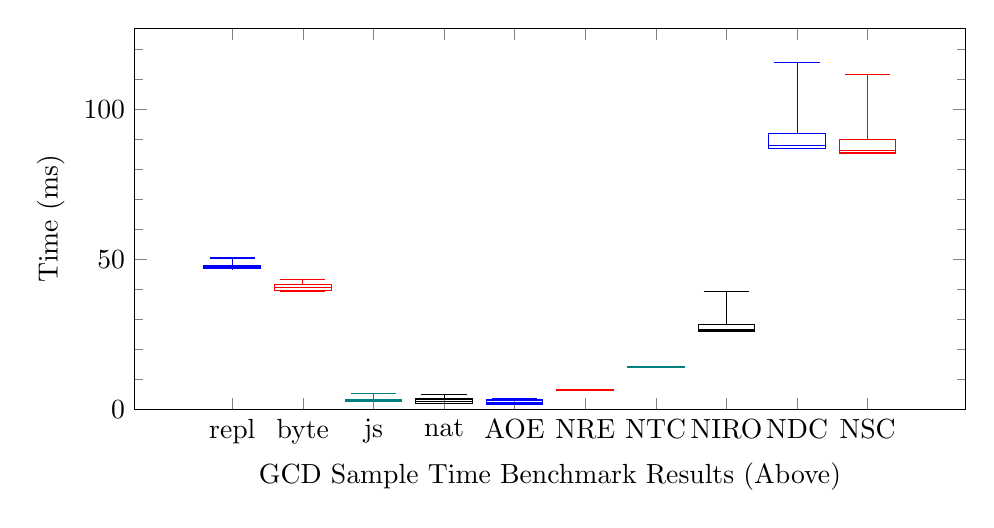
\begin{tikzpicture}
	\begin{axis}
	[
	width=\linewidth,
	height=0.53\linewidth,
	xlabel=GCD Sample Time Benchmark Results (Above),
	ylabel=Time (ms),
	boxplot/draw direction=y,
	xtick={1,2,3,4,5,6,7,8,9,10},
	xticklabels={repl, byte, js, nat, AOE, NRE, NTC, NIRO, NDC, NSC},
	minor y tick num=4,
	ymin=0,
	cycle list={{blue}, {red}, {teal}, {black}},
	]
	\addplot+[ boxplot prepared={lower whisker=46.916799999999995, lower quartile=46.9739690495893, median=47.54592600000001, upper quartile=48.11788295041072, upper whisker=50.520999999999994  }, ] coordinates {};
	\addplot+[ boxplot prepared={lower whisker=39.3934, lower quartile=39.629678719549936, median=40.625997999999996, upper quartile=41.622317280450055, upper whisker=43.497  }, ] coordinates {};
	\addplot+[ boxplot prepared={lower whisker=2.79998779297, lower quartile=2.79998779297, median=2.9419999122631992, upper quartile=3.3774727283827337, upper whisker=5.299997329710001  }, ] coordinates {};
	\addplot+[ boxplot prepared={lower whisker=2.0927, lower quartile=2.0927, median=2.6599920000000004, upper quartile=3.5743190467048436, upper whisker=5.004700000000001  }, ] coordinates {};
	\addplot+[ boxplot prepared={lower whisker=1.9, lower quartile=1.9, median=2.4459999999999997, upper quartile=3.2319287499512948, upper whisker=3.8  }, ] coordinates {};
	\addplot+[ boxplot prepared={lower whisker=6.4, lower quartile=6.453060024019196, median=6.528, upper quartile=6.602939975980803, upper whisker=6.7  }, ] coordinates {};
	\addplot+[ boxplot prepared={lower whisker=14.1, lower quartile=14.1, median=14.164000000000009, upper quartile=14.240837490847637, upper whisker=14.4  }, ] coordinates {};
	\addplot+[ boxplot prepared={lower whisker=26.2, lower quartile=26.2, median=26.657999999999987, upper quartile=28.4975749509059, upper whisker=39.5  }, ] coordinates {};
	\addplot+[ boxplot prepared={lower whisker=87, lower quartile=87, median=88.03, upper quartile=91.97703686326844, upper whisker=115.5  }, ] coordinates {};
	\addplot+[ boxplot prepared={lower whisker=85.5, lower quartile=85.5, median=86.38, upper quartile=90.03316301306162, upper whisker=111.5  }, ] coordinates {};
	\end{axis}
	\end{tikzpicture}
	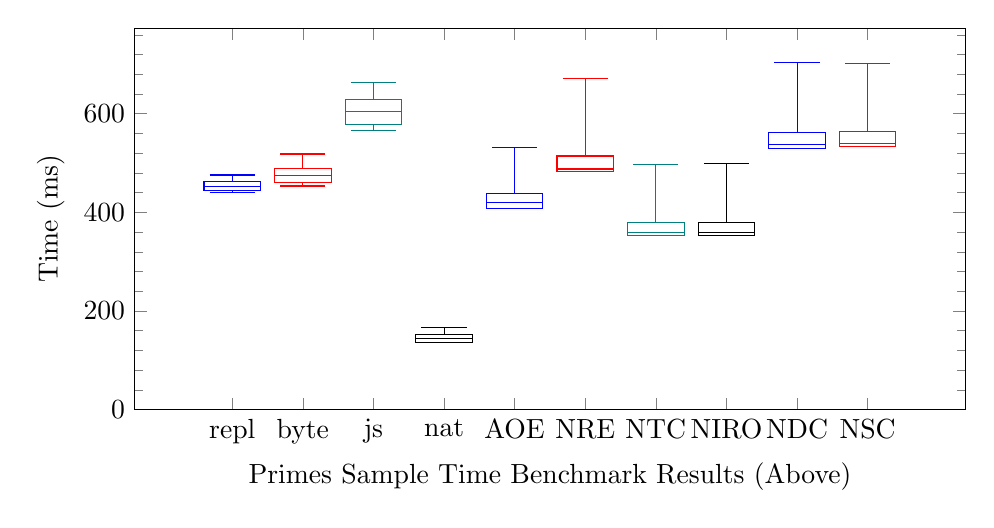
\begin{tikzpicture}
	\begin{axis}
	[
	width=\linewidth,
	height=0.53\linewidth,
	xlabel=Primes Sample Time Benchmark Results (Above),
	ylabel=Time (ms),
	boxplot/draw direction=y,
	xtick={1,2,3,4,5,6,7,8,9,10},
	xticklabels={repl, byte, js, nat, AOE, NRE, NTC, NIRO, NDC, NSC},
	minor y tick num=4,
	ymin=0,
	cycle list={{blue}, {red}, {teal}, {black}},
	]
	\addplot+[ boxplot prepared={lower whisker=440.0005, lower quartile=443.729268814417, median=453.1682800000001, upper quartile=462.60729118558316, upper whisker=475.711  }, ] coordinates {};
	\addplot+[ boxplot prepared={lower whisker=453.51750000000004, lower quartile=460.86905941993587, median=475.08469, upper quartile=489.3003205800642, upper whisker=518.2655000000001  }, ] coordinates {};
	\addplot+[ boxplot prepared={lower whisker=565.9999847400001, lower quartile=578.9949765768573, median=604.2200040816, upper quartile=629.4450315863427, upper whisker=663.4999513649999  }, ] coordinates {};
	\addplot+[ boxplot prepared={lower whisker=136.5105, lower quartile=136.6669762870124, median=144.18178999999998, upper quartile=151.69660371298755, upper whisker=167.15650000000002  }, ] coordinates {};
	\addplot+[ boxplot prepared={lower whisker=407, lower quartile=407, median=419.89, upper quartile=437.9297588675684, upper whisker=531  }, ] coordinates {};
	\addplot+[ boxplot prepared={lower whisker=482.5, lower quartile=482.5, median=487.88, upper quartile=514.2042397800961, upper whisker=672  }, ] coordinates {};
	\addplot+[ boxplot prepared={lower whisker=354, lower quartile=354, median=358.91, upper quartile=378.8871594577406, upper whisker=497  }, ] coordinates {};
	\addplot+[ boxplot prepared={lower whisker=354, lower quartile=354, median=358.49, upper quartile=378.5843997173342, upper whisker=498.5  }, ] coordinates {};
	\addplot+[ boxplot prepared={lower whisker=529, lower quartile=529, median=537, upper quartile=561.4989795705865, upper whisker=703  }, ] coordinates {};
	\addplot+[ boxplot prepared={lower whisker=533, lower quartile=533, median=540.28, upper quartile=563.855444852644, upper whisker=702  }, ] coordinates {};
	\end{axis}
	\end{tikzpicture}
	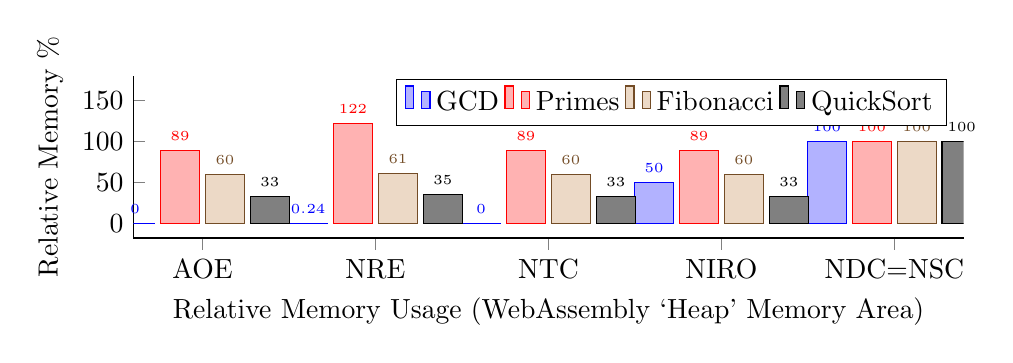
\begin{tikzpicture}
\begin{axis}
[
width=\linewidth,
height=0.3\linewidth,
xlabel=Relative Memory Usage (WebAssembly `Heap' Memory Area),
ylabel=Relative Memory \%,
xtick={1,2,3,4,5},
xticklabels={AOE, NRE, NTC, NIRO, NDC=NSC},
nodes near coords,
every node near coord/.append style={font=\tiny},
ybar,
ymax=180,
axis x line*=bottom,
axis y line*=left,
bar width = 0.5cm,
legend columns=4
]
%	\addplot coordinates {(1, 0) (2,0.012) (3, 0) (4, 2.49) (5, 4.97)};
%	\addplot coordinates {(1,314) (2,432) (3,314) (4,314) (5,356)};
%	\addplot coordinates {(1,11.9) (2,12.0) (3,11.9) (4,11.9) (5,19.9)};
%	\addplot coordinates {(1,26.9) (2,29.0) (3,26.9) (4,26.9) (5,82.3)};

\addplot coordinates {(1,0) (2,0.24) (3,0) (4,50) (5,100)};
\addplot coordinates {(1,89) (2,122) (3,89) (4,89) (5,100)};
\addplot coordinates {(1,60) (2,61) (3,60) (4,60) (5,100)};
\addplot coordinates {(1,33) (2,35) (3,33) (4,33) (5,100)};
\legend{GCD, Primes, Fibonacci, QuickSort}

\end{axis}
\end{tikzpicture}
	\caption{Time Benchmark Results for GCD and Primes, and Memory Benchmark Results. Box plots show the mean (middle line), one standard deviation either side (the box) and the minimum and maximum (whiskers).}
	\label{fig:timebenchgcdprime}
\end{figure}
\begin{figure}[p]
	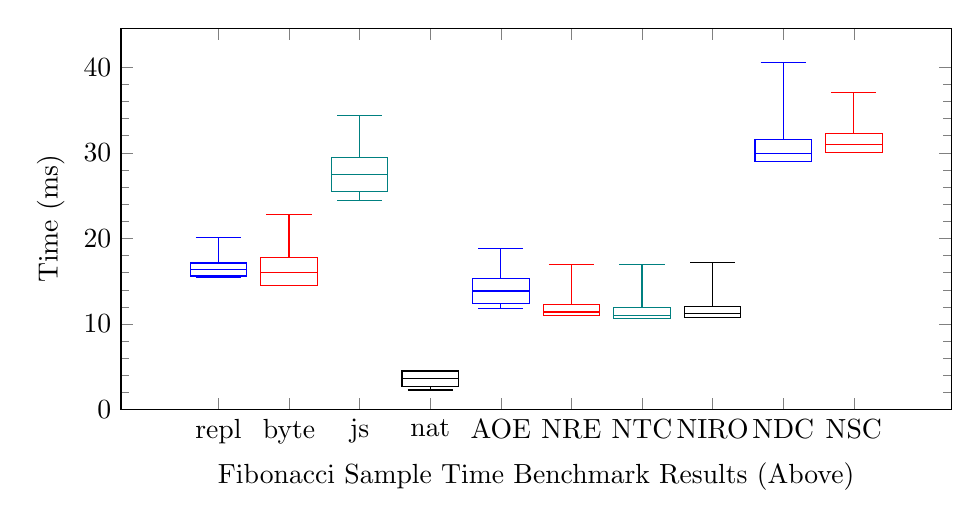
\begin{tikzpicture}
	\begin{axis}
	[
	width=\linewidth,
	height=0.53\linewidth,
	xlabel=Fibonacci Sample Time Benchmark Results (Above),
	ylabel=Time (ms),
	boxplot/draw direction=y,
	xtick={1,2,3,4,5,6,7,8,9,10},
	xticklabels={repl, byte, js, nat, AOE, NRE, NTC, NIRO, NDC, NSC},
	minor y tick num=4,
	ymin=0,
	cycle list={{blue}, {red}, {teal}, {black}},
	]
	\addplot+[ boxplot prepared={lower whisker=15.467199999999997, lower quartile=15.608607416911102, median=16.368972, upper quartile=17.129336583088897, upper whisker=20.128800000000002  }, ] coordinates {};
	\addplot+[ boxplot prepared={lower whisker=14.551600000000002, lower quartile=14.551600000000002, median=15.991112000000001, upper quartile=17.765839039365794, upper whisker=22.833000000000002  }, ] coordinates {};
	\addplot+[ boxplot prepared={lower whisker=24.399995803800003, lower quartile=25.483233126240698, median=27.460002899176, upper quartile=29.436772672111303, upper whisker=34.4000339508  }, ] coordinates {};
	\addplot+[ boxplot prepared={lower whisker=2.3004000000000002, lower quartile=2.6957899532811833, median=3.608784, upper quartile=4.521778046718817, upper whisker=4.6146  }, ] coordinates {};
	\addplot+[ boxplot prepared={lower whisker=11.8, lower quartile=12.43774826419513, median=13.86, upper quartile=15.282251735804868, upper whisker=18.8  }, ] coordinates {};
	\addplot+[ boxplot prepared={lower whisker=11, lower quartile=11, median=11.403999999999998, upper quartile=12.252989988162408, upper whisker=17  }, ] coordinates {};
	\addplot+[ boxplot prepared={lower whisker=10.6, lower quartile=10.6, median=11.036000000000003, upper quartile=11.915718136677851, upper whisker=17  }, ] coordinates {};
	\addplot+[ boxplot prepared={lower whisker=10.8, lower quartile=10.8, median=11.204000000000002, upper quartile=12.10065154881925, upper whisker=17.2  }, ] coordinates {};
	\addplot+[ boxplot prepared={lower whisker=29, lower quartile=29, median=29.89, upper quartile=31.53708834007165, upper whisker=40.5  }, ] coordinates {};
	\addplot+[ boxplot prepared={lower whisker=30, lower quartile=30, median=30.92, upper quartile=32.22904545375626, upper whisker=37  }, ] coordinates {};
	\end{axis}
	\end{tikzpicture}
	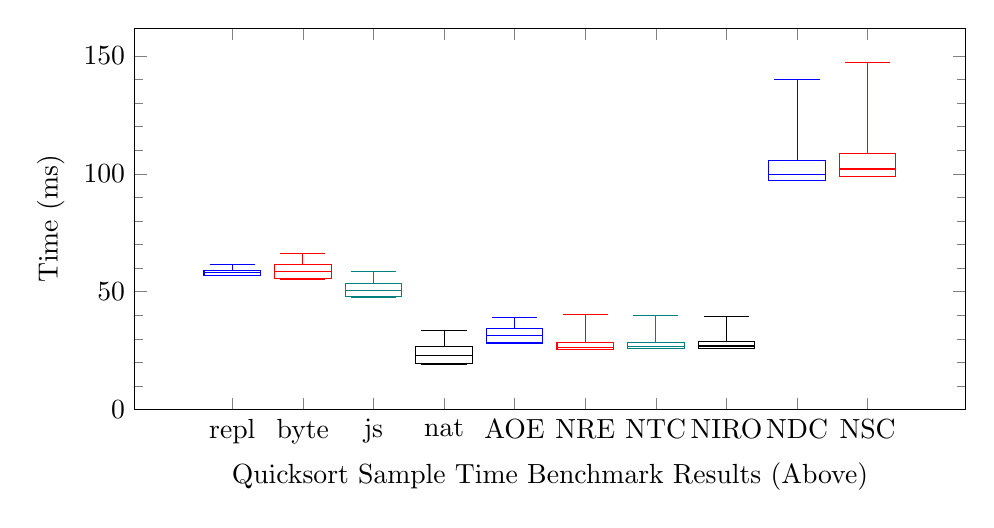
\begin{tikzpicture}
	\begin{axis}
	[
	width=\linewidth,
	height=0.53\linewidth,
	xlabel=Quicksort Sample Time Benchmark Results (Above),
	ylabel=Time (ms),
	boxplot/draw direction=y,
	xtick={1,2,3,4,5,6,7,8,9,10},
	xticklabels={repl, byte, js, nat, AOE, NRE, NTC, NIRO, NDC, NSC},
	minor y tick num=4,
	ymin=0,
	cycle list={{blue}, {red}, {teal}, {black}},
	]
	\addplot+[ boxplot prepared={lower whisker=56.8678, lower quartile=56.91425603242595, median=57.98698800000001, upper quartile=59.05971996757407, upper whisker=61.493599999999994  }, ] coordinates {};
	\addplot+[ boxplot prepared={lower whisker=55.09159999999999, lower quartile=55.52400983224097, median=58.515055999999994, upper quartile=61.50610216775902, upper whisker=66.2124  }, ] coordinates {};
	\addplot+[ boxplot prepared={lower whisker=47.399997711199994, lower quartile=47.85241953213496, median=50.64800262451201, upper quartile=53.44358571688906, upper whisker=58.399963379  }, ] coordinates {};
	\addplot+[ boxplot prepared={lower whisker=19.3928, lower quartile=19.423863834523758, median=23.019788000000002, upper quartile=26.615712165476246, upper whisker=33.4728  }, ] coordinates {};
	\addplot+[ boxplot prepared={lower whisker=28.2, lower quartile=28.289955717442474, median=31.31600000000001, upper quartile=34.342044282557545, upper whisker=39  }, ] coordinates {};
	\addplot+[ boxplot prepared={lower whisker=25.6, lower quartile=25.6, median=26.55199999999999, upper quartile=28.56418687004973, upper whisker=40.4  }, ] coordinates {};
	\addplot+[ boxplot prepared={lower whisker=26, lower quartile=26, median=26.667999999999996, upper quartile=28.60153975909475, upper whisker=40  }, ] coordinates {};
	\addplot+[ boxplot prepared={lower whisker=26, lower quartile=26, median=26.992000000000008, upper quartile=28.83415525947174, upper whisker=39.6  }, ] coordinates {};
	\addplot+[ boxplot prepared={lower whisker=97, lower quartile=97, median=99.54, upper quartile=105.46523417258754, upper whisker=140  }, ] coordinates {};
	\addplot+[ boxplot prepared={lower whisker=99, lower quartile=99, median=102.04, upper quartile=108.64896361012822, upper whisker=147  }, ] coordinates {};
	\end{axis}
	\end{tikzpicture}
	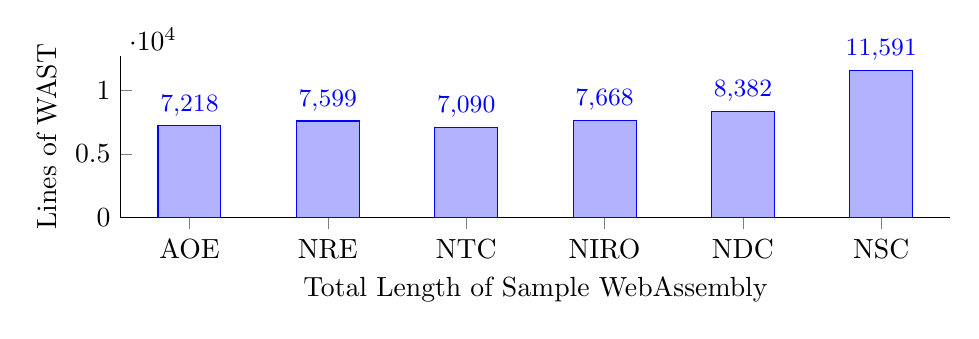
\begin{tikzpicture}
\begin{axis}
[
width=\linewidth,
height=0.3\linewidth,
xlabel=Total Length of Sample WebAssembly,
ylabel=Lines of WAST,
xtick={1,2,3,4,5,6},
xticklabels={AOE, NRE, NTC, NIRO, NDC, NSC},
nodes near coords,
every node near coord/.append style={font=\small},
ymin=0,
ybar,
axis x line*=bottom,
axis y line*=left,
bar width = 0.8cm,
]
%	\addplot coordinates {(1, 0) (2,0.012) (3, 0) (4, 2.49) (5, 4.97)};
%	\addplot coordinates {(1,314) (2,432) (3,314) (4,314) (5,356)};
%	\addplot coordinates {(1,11.9) (2,12.0) (3,11.9) (4,11.9) (5,19.9)};
%	\addplot coordinates {(1,26.9) (2,29.0) (3,26.9) (4,26.9) (5,82.3)};

\addplot coordinates {(1,7218) (2,7599) (3,7090) (4,7668) (5,8382) (6, 11591)};

\end{axis}
\end{tikzpicture}
	\caption{Time Benchmark Results for GCD and Primes, and Code Length Benchmark Results. Box plots show the mean (middle line), one standard deviation either side (the box) and the minimum and maximum (whiskers).}
	\label{fig:timebenchfibquick}
\end{figure}
\pagebreak
\section{Benchmark Results}
The results are promising: my compiler's WebAssembly is executed faster than the OCaml bytecode and Js\_of\_OCaml for all four benchmarks, and is hence a viable method for executing OCaml code on the web. There are however significant drawbacks: my code does not have to expend time performing garbage collection, and the lack of garbage collection means it is unlikely to be a good choice for executing high-memory-usage OCaml programs. Additionally, OCaml developers in practice use a standard library and split their code across multiple files, both features unsupported by my compiler and hence making it a more difficult to use tool for compiling OCaml for the web.
\\\\
Overall, the optimisations lead to significant speed-ups on all samples, with GCD's average execution time going from 86.4ms to 2.4ms, a reduction of 97\%. Primes' average execution time was reduced from 540.3ms to 419.9ms (22\% improvement), however with tail-call optimisation disabled this improves to 358.9ms (34\% improvement). There are many interesting observations to be made from the results for various optimisations:

\subsubsection{Stack Code Generation}
This optimisation clearly shows a significant line-of-code reduction of 28\% (measured from the original value) across all samples, although without a notable improvement in execution time. This is likely due to additional optimisations and compilation that WebAssembly goes under before it is executed: it must be compiled to register-based machine code, in practice removing the difference between accessing values on the stack and values stored in WebAssembly variables, both of which will likely become register accesses. In the case of GCD, we see execution time is slightly worsened with this optimisation, potentially a by-product of the stack code generator's ability to store a value on the stack for a long time until it is needed instead of storing it in a variable.

\subsubsection{Direct Calls}
Enabling this leads to a drastic improvement in execution time in all cases. GCD for instance executes in 26.5ms as opposed to 88ms. Memory usage also sees a great improvement due to the reduced need to construct closures as partial applications are replaced with full applications where possible. Finally, we also see a slight improvement in line-count, due to some memory operations for constructing closures being eliminated.

\subsubsection{IR Optimisations}
These only really effect the GCD sample, where dead-code elimination combined with tuple-load elimination leads to tuple-creation for the match statement being eliminated, thus reducing execution time and completely eliminating GCD's heap memory usage. In the other samples, alias-elimination can remove some variables and thus we see a reduction in the lines-of-code, but no improvement in execution time likely due to the WebAssembly environment's own optimisations when the WebAssembly is compiled to machine code.

\subsubsection{Tail Call Optimisation and Ref Elimination}
Enabling this optimisation cuts in half GCD's execution time compared to with just the previously discussed optimisations. However, for the other samples the result is either no improvement or an increase in execution time! A possible explanation for this is that GCD calls a tail-recursive function once that then loops many times, while other samples make many calls to tail-recursive functions that may loop only a few times, thus incurring the overhead of the loop and the `references' (eliminated with ref-elimination) without the gain if the loop is only used a few times. Primes for instance has mutually recursive functions that are tail-call optimised, but make frequent calls to each other.
\\\\
The increase in memory is due to the references, and is hence eliminated by ref-elimination. Lines-of-code also increases due to the additional loop code added to functions.

% TODO DONT FORGET ALL THE WORK IN MAKING THE CODE SHORTER

% TODO HOW IT WAS EVALUATED
% TODO TEST SYSTEM AND BENCHMARKS


\clearpage

\chapter{Conclusion}
%\note{This chapter is likely to be very short and it may well refer back to the Introduction. It might properly explain how you would have planned the project if starting again with the benefit of hindsight. }

%\note{
%	\begin{itemize}
%		\item SSA based IR?
%		\item More optimisations e.g. reverse copy-propagation, mutually recursive tail call optimisation, better match statements, better code generator that can re-order non side effecting instructions, speedy append implementation
%		\item More feature support: strings, records and mutable records, modules, named/optional function arguments, using the operators as function arguments (e.g. List.reduce ~f:(+) nums to sum a list)
%	\end{itemize}
%}

% TODO CONCLUDE THE DOCUMENT
% TODO IVE SUCCESSFULLY MET SUCCESS CRITERIA, SUMMARY OF EVERYTHING
% TODO WHAT LESSONS DID I LEARN
% TODO WHAT WORK COULD YOU DO IN THE FUTURE
\section{Outcome of the Project}
The project met and exceeded the success criteria: a subset of OCaml larger than the minimum sample specified in the proposal can be successfully compiled to WebAssembly, and several optimisations were implemented leading to a reduction in execution time varying from 22\% on the primes benchmark to 97\% on the GCD benchmark, consistently outperforming Js\_of\_OCaml as an option for running OCaml on the web.

\section{Lessons Learned}
Potentially the biggest lesson I learned was about the design of the intermediate representation (IR). Initially I implemented a stack-based, structured IR to make code generation simpler, but I later learned about the difficulties of optimising such an IR, hence switching to an unstructured, variable based IR, which set the project back by about a week at the end of January.

\section{Future Work}
There is a vast scope for potential future work on the project. One option would be to expand the subset of OCaml supported, by adding obviously useful features such as strings and records, or by supporting more nuanced features such as `guards' in match statement cases that allow a boolean condition to be checked before the case is taken. Work could be undertaken to support modules, which would open up the possibility of compiling multi-file programs and potentially to support using subsets of the standard library.
\\\\
Expanding the subset of features supported would also likely introduce interesting new avenues for optimisation --- for instance replacing a large string concatenation expression with something similar to Java's String Builders to avoid the $O(n^2)$ cost of the repeated concatenations. Of course even with the current subset, there are numerous further optimisations that could be implemented. Investigating which factors lead to a tail-call optimised function being faster could allow conditional operation of the tail-call optimiser to prevent functions such as those in the Prime benchmark from being converted.
\\\\
WebAssembly has a number of extensions in development --- for instance garbage collection. With the use of development versions of these extensions I could add support for garbage collection or exceptions, although this would make testing more challenging because my WebAssembly execution environment would need to support these extensions.

\clearpage

%%%%%%%%%%%%%%%%%%%%%%%%%%%%%%%%%%%%%%%%%%%%%%%%%%%%%%%%%%%%%%%%%%%%%
% the bibliography

\addcontentsline{toc}{chapter}{Bibliography}
\printbibliography[title={Bibliography}]
\clearpage

%%%%%%%%%%%%%%%%%%%%%%%%%%%%%%%%%%%%%%%%%%%%%%%%%%%%%%%%%%%%%%%%%%%%%
% the appendices
\appendix
% Assessors like to see some sample code or example circuit diagrams, and appendices are the sensible places to include such items. Accordingly, software and hardware projects should incorporate appropriate appendices. Note that the 12,000 word limit does not include material in the appendices, but only in extremely unusual circumstances may appendices exceed 10-15 pages - if you feel that such unusual circumstances might apply to you you should ask your Director of Studies and Supervisor to apply to the Chairman of Examiners. It is quite in order to have no appendices. Appendices should appear between the bibliography and the project proposal. 

\chapter{The Proposed Code Sample Appendix}

Things in appendix A / Code Samples? Examiners like to see some code samples, so maybe some of the following?
\begin{itemize}
	\item Mutually recursive value-binding type-checking routine (complex but commented nicely)
	\item Mutual recursion translation to IR
	\item Pattern matching IR implementation
	\item Reaching definitions implementation
	\item stack codegen is probably too complicated for examiners to understand the code easily? I wrote it and I have a hard time reading it
\end{itemize}


\clearpage

\chapter{The Intermediate Representation}
\thispagestyle{headings}
\label{chapter:ir}

%\begin{minted}{OCaml}
%type itype =
%| It_poly | It_bool | It_int | It_pointer | It_unit
%| It_float
%| It_none
%
%type iftype = itype * itype (* Function type *)
%type ituptype = itype list (* Tuple type *)
%
%type iunop =
%| Iun_neg (* Negate *)
%| Iun_eqz (* Equals zero *)
%
%type ibinop =
%| Ibin_add | Ibin_sub | Ibin_mul | Ibin_div | Ibin_rem (* Arithmetic *)
%| Ibin_and | Ibin_or (* Logic *)
%| Ibin_eq | Ibin_ne (* Equality *)
%| Ibin_lt | Ibin_le | Ibin_gt | Ibin_ge (* Comparison *)
%
%type iscope = Isco_local | Isco_global (* Variable scope *)
%
%type ivariable = iscope * string
%
%type iinstruction =
%(* Create a new var from a constant *)
%(* type of var, name of var *)
%| Iins_setvar of itype * ivariable * string
%(* Copy a var into another *)
%(* type of var, name of new var, name of old var *)
%| Iins_copyvar of itype * ivariable * ivariable
%(* Return var *)
%(* type of var, name of var *)
%| Iins_return of itype * ivariable
%(* Unary operation using one argument value *)
%(* type of operand, unary operation, result var, input var *)
%| Iins_unop of itype * iunop * ivariable * ivariable
%(* Binary operation using two argument values *)
%(* type of operands, binary operation *)
%| Iins_binop of itype * ibinop * ivariable * ivariable * ivariable
%(* Make a new closure for specified function and tuple type *)
%(* type of function, name of function, type of closure vars, result var *)
%| Iins_newclosure of iftype * string * ituptype * ivariable
%(* Fill a closure with a list of vars *)
%(* type of closure vars, name of var, list of vars to copy in *)
%| Iins_fillclosure of ituptype * ivariable * ivariable list
%(* Call closure in var, passing in an argument *)
%(* type of function, output var, closure var, var for argument *)
%| Iins_callclosure of iftype * ivariable * ivariable * ivariable
%(* Directly call a function, passing multiple arguments *)
%(* output var, name of function, type of args, arg vars *)
%| Iins_calldirect of ivariable * string * ituptype * (ivariable list)
%(* Start a block *)
%(* name of block *)
%| Iins_startblock of string
%(* End a block *)
%(* name of block *)
%| Iins_endblock of string
%(* Exit from the named block *)
%(* name of block *)
%| Iins_exitblock of string
%(* Exit from the named block if var is true *)
%(* name of block *)
%| Iins_exitblockif of string * ivariable
%(* Start an if statement *)
%(* name of block, condition var *)
%| Iins_startif of string * ivariable
%(* Else clause of an if statement *)
%(* name of block *)
%| Iins_else of string
%(* End an if statement *)
%(* name of block *)
%| Iins_endif of string
%(* Starts a loop, loops until an exitblock or exitblockif *)
%(* Name of escape block (to break to), name of loop block (to continue to) *)
%| Iins_startloop of string * string
%(* Ends a loop *)
%(* Name of break block, name of continue block *)
%| Iins_endloop of string * string
%(* Create a tuple of the given vars *)
%(* type of tuple, result var, argument vars *)
%| Iins_newtuple of ituptype * ivariable * ivariable list
%(* Load tuple's value at index i *)
%(* type of tuple, index in tuple, output var, tuple var *)
%| Iins_loadtupleindex of ituptype * int * ivariable * ivariable
%(* Create a construct of the given id and vars *)
%(* type of construct arguments, result var, id of construct, argument vars *)
%| Iins_newconstruct of ituptype * ivariable * int * ivariable list
%(* Load construct's value at index i *)
%(* type of construct arguments, index in arguments, output var, construct var *)
%| Iins_loadconstructindex of ituptype * int * ivariable * ivariable
%(* Load construct's ID *)
%(* output var, construct var *)
%| Iins_loadconstructid of ivariable * ivariable
%(* Create a mutable memory box for a value *)
%(* unboxed type, result var, var to box *)
%| Iins_newbox of itype * ivariable * ivariable
%(* Update a mutable memory box with a new value *)
%(* unboxed type, boxed var, unboxed var *)
%| Iins_updatebox of itype * ivariable * ivariable
%(* Load a value from a mutable memory box *)
%(* unboxed type, target var, boxed var *)
%| Iins_unbox of itype * ivariable * ivariable
%(* Fail, suspending execution *)
%(* No parameters *)
%| Iins_fail
%\end{minted}

\newcommand{\irone}[3]{\mathtt{Iins\_#1}(\mathtt{#2}_{#3})}
\newcommand{\irtwo}[5]{\mathtt{Iins\_#1}(\mathtt{#2}_{#3}, \mathtt{#4}_{#5})}
\newcommand{\irthree}[7]{\mathtt{Iins\_#1}(\mathtt{#2}_{#3}, \mathtt{#4}_{#5}, \mathtt{#6}_{#7})}
\newcommand{\irfour}[9]{\mathtt{Iins\_#1}(\mathtt{#2}_{#3}, \mathtt{#4}_{#5}, \mathtt{#6}_{#7}, \mathtt{#8}_{#9})}
\newcommand{\irtone}[3]{\mathtt{Iins\_#1}(\mathtt{type}_\tau, \mathtt{#2}_{#3})}
\newcommand{\irttwo}[5]{\mathtt{Iins\_#1}(\mathtt{type}_\tau, \mathtt{#2}_{#3}, \mathtt{#4}_{#5})}
\newcommand{\irtthree}[7]{\mathtt{Iins\_#1}(\mathtt{type}_\tau, \mathtt{#2}_{#3}, \mathtt{#4}_{#5}, \mathtt{#6}_{#7})}
\newcommand{\irtfour}[9]{\mathtt{Iins\_#1}(\mathtt{type}_\tau, \mathtt{#2}_{#3}, \mathtt{#4}_{#5}, \mathtt{#6}_{#7}, \mathtt{#8}_{#9})}
\newcommand{\mlist}[1]{#1\ \mathtt{list}}

%\vspace{-27pt}
\begin{flalign*}
\text{Basic Operations} & \\
& \irttwo{setvar}{result}{v}{constant}{c} \\
& \irttwo{copyvar}{dest}{v}{source}{v} \\
& \irtone{return}{source}{v} \\
& \irtthree{unop}{unop}{unop}{result}{v}{arg}{v} \\
& \irtfour{binop}{binop}{binop}{result}{v}{arg1}{v}{arg2}{v} \\
\text{Control} & \\
& \irone{startblock}{name}{block} \\
& \irone{endblock}{name}{block} \\
& \irone{exitblock}{name}{block} \\
& \irtwo{exitblockif}{name}{block}{condition\_var}{v} \\
& \irtwo{startif}{name}{block}{condition\_var}{v} \\
& \irone{else}{name}{block} \\
& \irone{endif}{name}{block} \\
& \irtwo{startloop}{break\_block}{block}{continue\_block}{block} \\
& \irtwo{endloop}{break\_block}{block}{continue\_block}{block} \\
& \mathtt{fail}() \\
\text{Memory} & \\
& \irthree{newtuple}{tuple\_type}{\mlist{\tau}}{dest}{v}{args}{\mlist{v}} \\
& \irfour{loadtupleindex}{tuple\_type}{\mlist{tau}}{index}{int}{result}{v}{tuple}{v} \\
& \irfour{newconstruct}{tuple\_type}{\mlist{tau}}{result}{v}{id}{int}{args}{\mlist{v}} \\
& \irfour{loadconstructindex}{tuple\_type}{\mlist{tau}}{index}{int}{result}{v}{construct}{v} \\
& \irtwo{loadconstructid}{result}{v}{construct}{v} \\
& \irttwo{newbox}{dest}{v}{arg}{v} \\
& \irttwo{updatebox}{box}{v}{arg}{v} \\
& \irttwo{unbox}{result}{v}{box}{v} \\
\text{Functions} & \\
& \irfour{newclosure}{func\_type}{\tau_{1} \rightarrow \tau_{2}}{name}{str}{cvar\_types}{\mlist{\tau}}{dest}{v} \\
& \irthree{fillclosure}{cvar\_types}{\mlist{\tau}}{closure}{v}{vars}{\mlist{v}} \\
& \irfour{callclosure}{func\_type}{\tau_{1} \rightarrow \tau_{2}}{result}{v}{closure}{v}{arg}{v} \\
& \irfour{calldirect}{result}{v}{func\_name}{str}{arg\_types}{\mlist{\tau}}{args}{\mlist{v}}
\end{flalign*}
\clearpage

\chapter{IR and WebAssembly Output of GCD}
\note{Tobias' proposal that I have an example program and show it at each step of the compilation. Could be a good idea but the code is massive, so this would easily extend to about 10+ pages. Also might require renaming some of the temporaries to make the code easier to read}
\note{Probably a bit much coming to think of it, so maybe just GCD sample, (untyped-AST?), IR and WebAssembly only to save from having to apply to the chairman of examiners for a longer appendix. I would rename temp variables to make the code easier to understand}

\section{OCaml}
The recursive GCD function as it is defined in the GCD sample.

\begin{minted}{OCaml}
let rec gcd a b =
  match (a, b) with
  | (0, y) -> y
  | (x, 0) -> x
  | _ ->
      if a > b then
        gcd (a - b) b
      else
        gcd (b - a) a
\end{minted}

\section{In IR Post-Optimisations}

The inner `gcd-app' function produced by compiling the above to the IR and then performing optimisations. Variable and block names have been changed to make the code easier to read.

\makeatletter
\expandafter\def\csname PYGdefault@tok@err\endcsname{\def\PYGdefault@bc##1{##1}}
\makeatother
\begin{minted}{Perl}
Function $$f_gcd-app:
-args:
$b_in (int)
-closure vars:
$a_in (int)
-local vars:
$a (int)
$b (int)
$a_copy (int)
$result (int)
$constant_zero_1 (int)
$a_ne_zero (bool)
$constant_zero_2 (int)
$b_ne_zero (bool)
$a_greater_than_b (bool)
$a_minus_b (int)
$b_minus_a (int)
-code:
copyvar int local.$a local.$a_in
copyvar int local.$b local.$b_in
startloop $break_loop $continue_loop
  copyvar int local.$a_copy local.$a
  startblock $match_block
    startblock $match_case_0_y
      setvar int local.$constant_zero_1 0
      binop int ne local.$a_ne_zero local.$a local.$constant_zero_1
      exitblockif $match_case_0_y local.$a_ne_zero
      copyvar int local.$result local.$b
      exitblock $match_block
    endblock $match_case_0_y
    startblock $match_case_x_0
      setvar int local.$constant_zero_2 0
      binop int ne local.$b_ne_zero local.$b local.$constant_zero_2
      exitblockif $match_case_x_0 local.$b_ne_zero
      copyvar int local.$result local.$a
      exitblock $match_block
    endblock $match_case_x_0
    startblock $match_case_default
      binop int gt local.$a_greater_than_b local.$a local.$b
      startif $if_a_greater_than_b local.$a_greater_than_b
        binop int sub local.$a_minus_b local.$a local.$b
        copyvar int local.$a local.$a_minus_b
        exitblock $continue_loop
      else $if_a_greater_than_b
        binop int sub local.$b_minus_a local.$b local.$a
        copyvar int local.$a local.$b_minus_a
        copyvar int local.$b local.$a_copy
        exitblock $continue_loop
      endif $if_a_greater_than_b
    endblock $match_case_default
    fail
  endblock $match_block
  exitblock $break_loop
endloop $break_loop $continue_loop
return int local.$result
\end{minted}

\section{WebAssembly}
The above IR code translated into WebAssembly.

\begin{minted}{LISP}
(func $$f_gcd-app (export "gcd")
  (param $a_in i32)
  (param $b_in i32)
  (result i32)
  (local $a i32)
  (local $b i32)
  (local $a_copy i32)
  (local $result i32)
    local.get $a_in
    local.set $a
    local.get $b_in
    local.set $b
    block $break_loop
      loop $continue_loop
        local.get $a
        local.set $a_copy
        block $match_block
          block $match_case_0_y
            local.get $a
            i32.const 0
            i32.ne
            br_if $match_case_0_y
            local.get $b
            local.set $result
            br $match_block
          end $match_case_0_y
          block $match_case_x_0
            local.get $b
            i32.const 0
            i32.ne
            br_if $match_case_x_0
            local.get $a
            local.set $result
            br $match_block
          end $match_case_x_0
          block $match_case_default
            local.get $a
            local.get $b
            i32.gt_s
            if $if_a_greater_than_b
              local.get $a
              local.get $b
              i32.sub
              local.set $a
              br $continue_loop
            else $if_a_greater_than_b
              local.get $b
              local.get $a
              i32.sub
              local.set $a
              local.get $a_copy
              local.set $b
              br $continue_loop
            end $if_a_greater_than_b
            br $match_block
          end $match_case_default
        unreachable
        end $match_block
        br $break_loop
      end $continue_loop
    end $break_loop
    local.get $result
)
\end{minted}
\clearpage

\chapter{Project Proposal}
\clearpage

\thispagestyle{empty}
	
	%\rightline{\large{Paul Durbaba}}
	%\medskip
	%\rightline{\large{Robinson}}
	%\medskip
	%\rightline{\large{pd452}}
    \rightline{\large{Candidate 2376D}}
	
	\vfil
	
	\centerline{\large Computer Science Tripos: Part II Project Proposal}
	\vspace{0.4in}
	\centerline{\Large\bf Compiling OCaml to WebAssembly}
	\vspace{0.3in}
	\centerline{\large{Friday 18\textsuperscript{th} October, 2019}}
	
	\vfil
	
	{\bf Project Originator:} Based on a proposal by Timothy Jones
	
	\vspace{0.1in}
	
	{\bf Resources Required:} See attached Project Resource Form
	
	\vspace{0.5in}
	
	{\bf Project Supervisor:} Tobias Kohn
	
	\vspace{0.2in}
	
	{\bf Signature:}
	
	\vspace{0.5in}
	
	{\bf Director of Studies:}  Alan Mycroft
	
	\vspace{0.2in}
	
	{\bf Signature:}
	
	\vspace{0.5in}
	
	{\bf Overseers:} Pietro Lio' and Robert Mullins
	
	\vspace{0.2in}
	
	{\bf Signatures:} 
	
	\vfil
	\eject
	
	
	\section*{Introduction and Description of the Work}
	The aim of the project is to implement a compiler from a subset of OCaml to WebAssembly.
	\\\\
	WebAssembly\footnote{https://webassembly.org/} is a binary instruction format for the web with the main goal of improving performance of more computationally intensive functions in web applications. It does not replace JavaScript as there (currently) is no way to perform tasks such as DOM manipulation directly from WebAssembly - it is expected that a JavaScript application might call some functions implemented in WebAssembly to perform computation, and then display the results itself.
	\\\\
	My work will involve writing a compiler in OCaml and a runtime system in a language such as C. 
	\\\\
	The compiler will take an AST (abstract syntax tree) produced by the lexer and parser of the OCaml compiler\footnote{https://github.com/ocaml/ocaml} (ocaml-compiler-libs), performing type checking (I considered using the OCaml type checker, but getting that to work might be just as hard as writing my own type checker), and then transforming the typed AST through a series of intermediate representations (IRs). Each IR will eliminate some higher-level feature, for instance replacing first-class functions with closures. At the end, I will generate instructions to target WebAssembly. The WebAssembly Binary Toolkit\footnote{https://github.com/WebAssembly/wabt} will then be used to output a usable WebAssembly module.
	\\\\
	The runtime system will be needed to implement closures and memory allocation / access in a way that can be used by the code generated by my compiler.
	
	\section*{Starting Point}
	\subsection*{OCaml and Compilers}
	I have done very little programming in OCaml previously, with the exception of coming up with some code samples when considering which features this compiler should support. However I have some experience in programming in Standard ML, a similar language, from Part IA Foundations of Computer Science.
	\\\\
	I also have little previous experience in writing compilers. I have written basic lexers and parsers, and implemented a system for interpreting mathematical expressions, however I have no experience with a larger compiler that compiles to instructions instead of interpreting.
	
	\subsection*{WebAssembly and the Web}
	I have no experience with WebAssembly with the exception of reading through some of the documentation in the weeks leading up to this proposal.
	\\\\
	I have a fair amount of experience with JavaScript and websites: I do not anticipate any issue with coming up with a suitable demonstration of the WASM produced by the compiler.
	
	
	\section*{Substance and Structure of the Project}
	
	%KEY CONCEPTS, MAJOR WORK ITEMS, THEIR RELATIONS AND RELATIVE IMPORTANCE, DATA STRUCTURES AND ALGORITHMS
	
	%Key Concepts: Type Checking, WebAssembly, Runtime System, Closure
	%Major Work Items: Components
	%Relative importance: All important!
	
	%Data Structures: Trees, lots of trees!

	The main components of the compiler are the type checker, the intermediate representations, the WebAssembly code generator, and the runtime system. These will need to be implemented in the order listed, as each depends on the last, with the exception of the runtime system and code generator which can be developed in parallel, as a change in one might require a change in the other. Likewise, they are all equally important in a complete compiler, as each part is required during the translation from AST through to a WebAssembly module.
	\\\\
	My subset of OCaml will include the following:
	\begin{itemize}
		\item Values: \camlinline{int} (64-bit signed integer), \camlinline{bool} and \camlinline{float} (64-bit floating point), able to be defined using expressions \camlinline{let} and \camlinline{let ... in}.
		\item Functions: \camlinline{let} and \camlinline{let rec} with multiple curried arguments, with an expression for the function body, as well as inline functions using \camlinline{fun}
		\item Types: Non-polymorphic types defined using \camlinline{type}, and tuples. These can be used to implement list types, and hence lists themselves will not be part of the subset (although supporting list syntax will be an extension)
		\item \camlinline{if ... then ... else} and basic pattern matching. I was planning on excluding pattern matching from the initial subset, however it is needed to match types and de-structure them, and alternate approaches would lead to clumsy syntax. Pattern matching will be limited to use on types.
	\end{itemize}
	Polymorphism is excluded from the initial subset as I do know how challenging to implement it will be, however it will likely be the first stretch goal that I try and implement.

	\subsection*{Testing}
	I intend to write unit tests, for instance using the OUnit\footnote{https://github.com/gildor478/ounit} unit testing framework. These will function to demonstrate that sub-components are working before the whole compiler can be tested, and more importantly to prevent the re-introduction of bugs that have already been fixed by writing a unit test when a bug is found to ensure it doesn't occur again.
	\\\\
	The overall compiler will be tested with a selection of code samples designed to test important features and edge cases. The compiled code will be executed in the browser and the result checked against the expected result. This could also be automated, e.g. by using a WebAssembly interpreter such as the WebAssembly reference interpreter\footnote{https://github.com/WebAssembly/spec/tree/master/interpreter}, depending on the complexity of this.
	
	\subsection*{Evaluation}
	I will evaluate my compiler in comparison to other methods of executing OCaml, particularly on the web, such as the OCaml compiler and Js\_of\_ocaml\footnote{https://ocsigen.org/js\_of\_ocaml/3.1.0/manual/overview}. I will do this by measuring performance in terms of how long particular samples of OCaml code take to execute on these different platforms, by running them multiple times on each platform (or the sample includes a loop of the same effect), and recording the time between execution starting and execution completing.
	\\\\
	It would also be interesting to compare memory usage between the different approaches, however that will likely be unfeasible due to the difficulty of getting accurate memory usage statistics, e.g. how much of the browser's memory is used by the JavaScript OCaml interpreter.
	\\\\
	When optimisations are implemented, I will analyse the performance with and without the optimisation, for instance by using timing facilities available in JavaScript. An optimisation will be considered successful if it leads to a measurable increase in execution speed (or a measurable decrease in memory usage) for a carefully chosen set of OCaml programs.
	
	
	\section*{Success Criterion}
	The project will be a success if the following criteria are met:
	\begin{itemize}
		\item The compiler can take a selection of reasonable (not likely to result in more than 10MB of memory allocation) samples written using all features of the selected subset of OCaml, and compile them to WebAssembly modules
		\item These WebAssembly modules can be loaded and executed with a set of provided input values for each sample in the latest version of Chrome and Firefox to produce the same results as if the OCaml code they were compiled from was compiled, executed, and given the same input value by the OCaml Compiler
	\end{itemize}
	
	
	\section*{Possible Extensions}
	% Pattern Matching, References and Loops, Garbage Collection, Exceptions,
	\begin{itemize}
		\item Expanding my subset of OCaml supported: polymorphism, more advanced pattern matching, list syntax, strings, references, for and while loops, modules...
		
		\item Improving code access from JavaScript, for instance allowing JavaScript objects (probably just numbers and strings) to be passed to OCaml functions, likely with a special type to represent JavaScript objects
		
		\item Optimisations: There are many optimisations that could be implemented to improve the code generated by the compiler, for instance peephole optimisation, dead-code elimination, constant propagation, function call inlining, and many more that I could learn about.
		
		\item End to End testing: Using a WebAssembly interpreter, whereby I can specify a sample of programs to compile, and the expected output from running them, and validate that they all compile and produce the expected results in the interpreter.
		
		\item Supporting Exceptions. This would be challenging due to WebAssembly's current lack of support for them, however there are ways of working around this, with their own performance costs. One way might be to make functions that throw exceptions return a type that signifies either a result or an exception was thrown, then we can check if an exception was thrown after each function call, and propagate exceptions until a relevant catch block is found.
		
		\item Garbage Collection. WebAssembly likewise does not currently support garbage collection, and additionally does not allow walking the stack for security reasons. There are limited ways to work around this: by storing all values except for primitive types and references on the heap, reference counting could be used to track which heap items have references on the stack, and tracing could be used between heap items. A system like this would likely have to be implemented in JavaScript or TypeScript due to the complexity of getting it right in WebAssembly.
		
	\end{itemize}
	
	\section*{Timetable and Milestones}
	
	\subsection*{25th Oct - 8th Nov}
	Getting ready:
	\begin{itemize}
		\item Creating a git repository and GitHub remote for the project, and skeleton for the overall project
		\item Setting up the required libraries (the ocaml-compiler-libs)
		\item Setting up and trying out unit testing with OUnit
		\item Parsing OCaml files using the ocaml-compiler-libs parser, and experimenting with the resulting ASTs to learn more about them 
	\end{itemize}
	In addition, I will practice coding in OCaml to learn more about the language and come up with useful code samples that will be useful for testing later on. The book \textit{Types and Programming Languages} by Benjamin C. Pierce contains some OCaml samples to help me learn and also prepare me for writing the type checker.
	
	\subsection*{9th Nov - 22nd Nov}
	I will implement a type checker for the initial subset of OCaml. If I have time, polymorphism (an extension) could also be implemented at this stage, certainly my implementation of type checking will have to consider how polymorphism will be implemented in the future.
	\\\\
	At the end of this I should have a function that can take an OCaml AST and output a typed AST, with a type attached to each node.
	
	\subsection*{23nd Nov - 6 Dec}
	Implement translation of the typed AST through to a lower-level representation suitable for transformation into WebAssembly instructions.
	
	\subsection*{7 Dec - 20 Dec}
	Implement code generation and a suitable runtime system for WebAssembly to perform memory allocation and closure calls, probably using C. After this point, it should be possible to use the compiler to compile some code samples and execute them in a browser, and hence I will have met my success criterion.
	
	\subsection*{20 Dec - 3 Jan}
	I will probably be taking about a week's break from the project, and using the remaining time in these two weeks to clean up / improve the project if the success criterion has been met (for instance by refactoring, implementing additional test cases or adding better error messages), and continue working up to the success criterion otherwise.
	
	\subsection*{4 Jan - 17 Jan}
	I will implement polymorphism in the type checker and some form of polymorphism elimination in the intermediate representation. I also hope to implement references and for/while loops, which should be fairly simple to implement but will allow more interesting programs to be compiled.
	
	\subsection*{17 Jan - 31 Jan}
	I will implement some optimisations such as the ones I listed above, and evaluate them as I described in the evaluation section.
	\\\\
	Write the progress report.
	
	\subsection*{1 Feb - 14 Feb}
	Presentations and preparation needed for them.
	\\\\
	I will investigate and implement some way of passing JavaScript values (numbers and strings) to functions, and seek to improve my pattern matching implementation by compiling more complicated match statements.
	
	\subsection*{15 Feb - 28 Feb}
	I will set up an end to end testing system as described in the stretch goals section.
	
	\subsection*{1 Mar - 13 Mar}
	Start writing dissertation. Investigate supporting exceptions and garbage collection - perhaps the WebAssembly extensions to support them will be finished by this time. I will decide to work on either exceptions, garbage collection or additional optimisations, depending on the complexity of supporting exceptions or garbage collection.
	
	\subsection*{14 Mar - 27 Mar}
	Continue writing dissertation. Attempt to wrap up remaining unfinished features e.g. those I started in the last two weeks.
	
	\subsection*{28 Mar - 10 Apr}
	Continue with the dissertation, submitting first drafts of chapters to my supervisor. Focus on improving the code e.g. by refactoring, or implementing additional tests.
	
	\subsection*{10 Apr - 24 Apr}
	Fully focus on the dissertation, leaving the code as it is. Submit draft version of dissertation to supervisor and DoS.
	
	\subsection*{24th Apr - 8 May}
	At this point the dissertation should be complete, with only minor changes to be made over these weeks.
	\\\\
	Towards the end of these two weeks, I will submit the final version of my dissertation.
	
	
	\section*{Resource Declaration}
	I plan to do the work via remote desktop to my server located in France, so I can easily switch between using my desktop and laptop. This has 32GB RAM and two 2 TB HDDs in RAID 1 (mirrored). I will use git for version control of code and important documents, which will be regularly pushed to a private GitHub repository. In addition, both my laptop and desktop automatically download backups of data on my server at regular intervals when they are online.
	\\\\
	I accept full responsibility for this machine and I have made contingency plans to protect myself against hardware and/or software failure.
	\\\\
	I will be making use of some components of the OCaml compiler (the lexer, parser, and possibly type-checker), as well as the WebAssembly Binary Toolkit (WABT).

\end{document}
